\documentclass[output=paper]{langscibook}

\author{Cherry Chit-Yu Lam \affiliation{University of Cambridge}}
\title{Croft's Cycle in Mandarin and Cantonese throughout history and across varieties} 
\shorttitlerunninghead{Croft's Cycle in Mandarin and Cantonese}

\abstract{One of the oldest problems in Chinese linguistics is negation and currently there is no consensus on a theory for the distribution of negators. This article explores this issue from the perspective of Croft's Negative Existential Cycle (NEC) based on diachronic evidence and synchronic comparative data from four varieties of Chinese. The results show that the NEC is attested in Chinese throughout its history and across all varieties, and that different varieties can be positioned at different stages in the Cycle. The shared historical origin of the Mandarin \textit{méi(yǒu)}, the Hong Kong Cantonese \textit{mou5} and the Gaozhou Cantonese \textit{mau5}, and their involvement in the NEC account for their semantic similarity in producing a non-existence reading as a standard negator. They also provide a new understanding of the nature of these negators and their present-day structural behaviour.

\textbf{Keywords:} varieties of Chinese, non-existence, perfectivity, standard negation}


\begin{document}
\maketitle

\section{Introduction}\label{s:lam1}

Negation in Chinese, particularly \ili{Mandarin Chinese}, has received considerable attention in the last half century. Researchers in the field are keenly interested in solving the puzzle regarding the distribution of two Mandarin negators \textit{bù} `not' and \textit{méi(yǒu)} `not (have)'. The mainstream understanding thus far is that \textit{méi(yǒu)} is a special negator for perfective sentences because they refer to terminated or even finished situations, while \textit{bù} is a `neutral/general' negator that applies to all other conditions as the `elsewhere' strategy as suggested in \cite{LiThompson1981}. However, there is little consensus on the reasons for this division of labour in Mandarin negation. This study offers a diachronic-comparative analysis of Chinese negation from the perspective of \citeauthor{Croft1991}'s Negative Existential Cycle (NEC). I argue that the standard negation in Chinese has a strong connection to its negative existential construction as suggested in \citeauthor{Croft1991}'s (\citeyear{Croft1991}) original proposal. Therefore, this analysis serves three purposes. Firstly, it provides a new understanding of the overall architecture of the Chinese negation system, where negators such as \textit{méi(yǒu)} are not perfective negators but negators of existence. This conclusion is inspired by the NEC, which provides a model for the connection between standard negation and existential negation. Secondly, the diachronic study of Chinese negation offers further evidence for the attestation of the NEC as a diachronic model (see the work by Veselinova on Uralic, Slavonic and Polynesian languages). Based on the typological findings reported in \cite{Veselinova2014}, a system (such as Polynesian) may require as long as two thousand years to complete the entire NEC. For this reason, Chinese is a strong candidate for testing \citeauthor{Croft1991}'s NEC on actual diachronic data owing to the long history and extensive documentation of the Chinese language. Thirdly, this analysis constitutes a comparative study on four Chinese varieties: Beijing Mandarin, Taiwan Mandarin, Hong Kong Cantonese, and Gaozhou Cantonese.\footnote{Glottocode from glottolog 3.0: Beijing Mandarin (Sino-Tibetan, Sinitic, […] Northern Chinese, Mandarinic, Mandarin Chinese, Beijingic) [beij1234]

Taiwan Mandarin (Sino-Tibetan, Sinitic, […] Northern Chinese, Mandarinic, Mandarin Chinese, Beijingic) [taib1240]

Hong Kong Cantonese (Sino-Tibetan, Sinitic, […] Yue-Pinghua, Yue Chinese, Yuehai, Cantonese) [xian1255]} 
The latter is a scarcely documented and un(der)-studied Cantonese variety spoken in Maoming, a south-western county in the Guangdong Province of China. The main objective of this analysis is to determine how the NEC can apply to various Chinese varieties and how different varieties display properties of different stages in the Cycle.\footnote{All Mandarin examples have been romanised using Hanyu Pinyin, and all Cantonese examples with Jyutping. Tones are marked on the lexical items that are mentioned in the text and tables, but not in the examples.} 

The article proceeds as follows. §\ref{s:lam2} presents the key features of Chinese negation and illustrates the relevance of the NEC to Chinese. Then §\ref{s:lam3} focuses on the situation in Mandarin by first introducing historical evidence that demonstrates the development in the expression of the negative existential from Old Chinese to Pre-modern Mandarin, and then accounts for the emergence of \textit{méi(yǒu)} as the standard negator in present-day Mandarin. In §\ref{s:lam4}, I examine the two Cantonese varieties and discuss the variation observed among the four Chinese varieties as well as the key implications of this comparative study. Finally, conclusions are presented in §\ref{s:lam6}. %\todo{section 5 is missing in the roadmap}

\section{Background and methodology}\label{s:lam2}
\subsection{The Chinese negation puzzle}\label{s:lam2-1}

This section presents the background of standard negation in the Chinese language. Standard negation is defined here as the construction that applies to the most basic verbal declarative main clause to reverse the truth value of the proposition that the clause expresses (\citealt{Miestamo2005}). The marker used to perform such function is known as a `standard negator', such as `not' in \textit{Lucy does \textbf{not} swim}. Modern Mandarin Chinese has two standard negators, \textit{bù} `not' and \textit{méi(yǒu)} `not (have)', and both appear between the subject and the verb. Their distributional properties can be illustrated as follows. 

In a simple verbal declarative clause without aspect-marking (henceforth `bare sentence', which is also referred to as a `plain sentence' in \citealt{Wang1965}) such as the clause in example (\ref{ex:lam1a}), the default negative form is constructed by inserting \textit{bù} `not' immediately preceding the verb (\ref{ex:lam1b}). This reverses the meaning of what the proposition in the affirmative claims. In this case, it denies that the speaker buys books. I will refer to the negative form of bare sentences as the `bare negative', for the absence of overt aspect-marking or any type of adverbial modification.

% \todo{Had some problems with Chinese font so boldface is not working right now, but will hopefully be able to solve it.}

\ea Mandarin (Mandarinic, Sinitic) \label{ex:lam1}\\ 
  \ea {\cn 我買書} \label{ex:lam1a}\\
    \gll wo mai	shu \\
         I	buy	book\\
    \glt `I buy books.'
  \ex {\cn 我\textbf{不}買書} \label{ex:lam1b}\\
    \gll wo \textbf{bu} [mai shu]\\
    	I \textbf{not} buy book\\
    \glt `I do not buy books.'
\z \z

The system becomes more complicated when aspect-marking is present. Examples (\ref{ex:lam2}-\ref{ex:lam3}) contain the negation pattern in Mandarin when the verb \textit{mǎi} `to buy' is marked with perfective and experiential aspect, respectively. The sentences (\ref{ex:lam2b}) and (\ref{ex:lam3b}) illustrate the unmarked strategy for negating the affirmative sentences in (\ref{ex:lam2a}) and (\ref{ex:lam3a}). In short, whenever the affirmative sentence is perfectively marked either as perfective or experiential, \textit{méiyǒu} is used instead of \textit{bù} (see examples \ref{ex:lam2d} and \ref{ex:lam3c}). One important difference between the negation of perfective sentences and that of experiential sentences is the co-occurrence constraint on the negator and the aspect marker – \textit{méiyǒu} can co-occur with the experiential marker \textit{guo} (\ref{ex:lam3b}), but not with the perfective marker \textit{le}, as shown in example (\ref{ex:lam2c}). 

\ea Mandarin negation and perfective aspect \label{ex:lam2}\\
  \ea {\cn 我買\textbf{了}書} \label{ex:lam2a}\\
    \gll wo	mai-\textbf{le} shu \\
    I buy-\textbf{\textsc{pfv}} book\\
    \glt `I bought books.'
  \ex {\cn 我\textbf{沒有}買書} \label{ex:lam2b}\\
    \gll wo	\textbf{mei-you} mai shu \\
    I \textbf{not-have} buy book\\
    \glt `I did not buy books.'
  \ex {\cn 我\textbf{沒有}買\textbf{了}書} \label{ex:lam2c}\\
  	\gll *wo	 \textbf{mei-you} mai-\textbf{le} shu\\
  	I \textbf{not-have} buy-\textbf{\textsc{pfv}} book\\
  	\glt Intended: `I did not buy books.'
  \ex {\cn 我\textbf{不}買\textbf{了}書} \label{ex:lam2d}\\
  	\gll *wo	 \textbf{bu} mai-\textbf{le} shu \\
  	I \textbf{no}t buy-\textbf{\textsc{pfv}} book\\
  	\glt Intended: `I did not buy books.'
\z \z


\ea Mandarin negation and experiential aspect \label{ex:lam3}\\
  \ea {\cn 我買\textbf{過}書} \label{ex:lam3a}\\
    \gll wo	mai-\textbf{guo} shu\\
	I buy-\textbf{\textsc{exp}} book\\
	\glt `I have bought books (before).'
  \ex {\cn 我\textbf{沒有}買\textbf{過}書} \label{ex:lam3b}\\
    \gll wo	\textbf{mei-you} mai-\textbf{guo} shu\\
	I \textbf{not-have} buy-\textbf{\textsc{exp}} book\\
	\glt `I have not bought books (before).'
  \ex {\cn 我\textbf{不}買\textbf{過}書} \label{ex:lam3c}\\
  \gll *wo \textbf{bu} mai-\textbf{guo} shu \\
  	I \textbf{not} buy-\textbf{\textsc{exp}} book\\
  	\glt Intended: `I have not bought books (before).'
\z \z

This is the Chinese negation puzzle, and while this puzzle confirms that both \textit{bù} and \textit{méi(yǒu)} are standard negators in Mandarin, it also raises two issues. Firstly, Mandarin appears to have a neat system wherein the distribution of the negators is conditioned by the presence of aspect markers. Contrasting example (\ref{ex:lam1}) with (\ref{ex:lam2}-\ref{ex:lam3}), \textit{bù} fails to perform its negator function when an affirmative sentence is aspect-marked; the only appropriate negator is \textit{méi(yǒu)}. \cite{Huang1988} suggested that \textit{bù} cannot co-occur with perfective markers because \textit{bù} must cliticise onto the verb first, but marking a non-event (an event already negated or denied) as completed or realised would result in semantic anomaly. In other words, the incompatibility is a matter of interpretation that stems from the narrow scope of negation. \cite{Ernst1995} proposed that due to the unboundedness requirement of \textit{bù} – meaning that \textit{bù} has an intrinsic requirement to select for an unbounded situation as its complement – it is unacceptable in the presence of perfective markers. In short, a terminated or completed event would be incompatible with \textit{bù}. \cite{Lin2003} made a similar suggestion by stating that \textit{bù} requires its complement to be a stative situation that does not require further energy input. \cite{Li2007} in turn has adopted a feature-checking approach to account for negation-aspect compatibility. She proposes that both aspect markers and negators possess the same four atomic aspectual features, but different markers have different inherent values for these features, and their compatibility is a result of their feature compatibility. 

The second issue concerns the intriguing connection between \textit{méi(yǒu)} `not (have)' and perfective aspect. As demonstrated in the examples above, \textit{méi(yǒu)} can occur with the experiential marker \textit{guo} (\ref{ex:lam3b}) but not with the perfective marker \textit{le} as in example (\ref{ex:lam2c}). \cite{Wang1965} is the first to propose that \textit{yǒu} `have' in \textit{méi(yǒu)} and \textit{le} are morphological alternants in complementary distribution, with the former appearing in negative contexts and the latter only in affirmatives. The morphological connection between \textit{yǒu} and \textit{le} has been challenged by \citet[434--438]{LiThompson1981} as well as \cite{Li2007}, but the assumption that \textit{yǒu} is an aspectual auxiliary (or a perfective auxiliary) has remained widely adopted in subsequent studies on Mandarin negation.

The position that negation has a close relationship with temporality is not new (see \citealt{Zanuttini2001} and \citealt{Miestamo2005}), and the suggestion that aspect is the temporal system to which negation is connected in Chinese is exceedingly plausible as well, because aspect is the most prominently and overtly formalised temporal category in Chinese. Indeed, the same negation-aspect compatibility pattern is also identified in the two Cantonese varieties investigated in this paper – Hong Kong and Gaozhou Cantonese. Examples (\ref{ex:lam4}) to (\ref{ex:lam9}) adopt the sentences from example (\ref{ex:lam1}) and present the corresponding structures in the two Cantonese varieties.

\ea Hong Kong Cantonese \label{ex:lam4}\\
  \ea {\cn 我買書} \label{ex:lam4a}\\
    \gll ngo	mai	syu\\
	I buy book\\
	\glt `I buy books.'
  \ex {\cn 我\textbf{唔}買書} \label{ex:lam4b}\\
    \gll ngo	 \textbf{m} [mai syu]\\ 
	I \textbf{not} buy book\\
	\glt `I do not buy books.'
\z \z


\ea Hong Kong Cantonese negation and perfective aspect \label{ex:lam5}\\
  \ea {\cn 我買咗書} \label{ex:lam5a}\\
    \gll ngo mai-\textbf{zo} syu\\
	I buy-\textbf{\textsc{pfv}} book\\
	\glt `I bought books.'
  \ex {\cn 我冇買書} \label{ex:lam5b}\\
    \gll ngo \textbf{mou} mai syu\\
	I \textbf{not.have} buy book\\
	\glt `I did not buy books.'
  \ex {\cn 我冇買咗書} \label{ex:lam5c}\\
  	\gll *ngo \textbf{mou} mai-\textbf{zo} syu\\
	I \textbf{not.have} buy-\textbf{\textsc{pfv}} book\\
	\glt Intended: `I did not buy books.'
  \ex {\cn 我\textbf{唔}買咗書} \label{ex:lam5d}\\
  	\gll *ngo \textbf{m} mai-\textbf{zo} syu\\
  	I \textbf{not} buy-\textbf{\textsc{pfv}} book\\
  	\glt Intended: `I did not buy books.'
\z \z


\ea Hong Kong Cantonese negation and experiential aspect \label{ex:lam6}\\
  \ea {\cn 我買\textbf{過}書} \label{ex:lam6a}\\
  	\gll ngo mai-\textbf{gwo} syu\\
	I buy-\textbf{\textsc{exp}} book\\
	\glt `I have bought books (before).'
  \ex {\cn 我冇買\textbf{過}書} \label{ex:lam6b}\\
  	\gll ngo \textbf{mou} mai-\textbf{gwo} syu \\
  	I \textbf{not.have} buy-\textbf{\textsc{exp}} book\\
  	\glt `I have not bought books (before).'
  \ex {\cn 我\textbf{唔}買\textbf{過}書} \label{ex:lam6c}\\
	\gll *ngo \textbf{m} mai-\textbf{gwo} syu\\
  	I \textbf{not} buy-\textbf{\textsc{exp}} book\\
	\glt Intended: `I have not bought books (before).'
\z\z


\ea Gaozhou Cantonese \label{ex:lam7}\\
  \ea {\cn 我買書} \label{ex:lam7a}\\
  	\gll ngo	mai	syu\\
  	I buy book\\
	\glt `I buy books.'
  \ex {\cn 我茅買書} \label{ex:lam7b}\\
  	\gll ngo \textbf{mau} [mai syu]\\
  	I \textbf{not} buy book\\
  	\glt `I do not buy books.'
\z\z


\ea Gaozhou Cantonese negation and perfective aspect \label{ex:lam8}\\
  \ea {\cn 我買\textbf{嗲}書} \label{ex:lam8a}\\
  	\gll ngo mai-\textbf{de} syu\\
  	I buy-\textbf{\textsc{pfv}} book\\
 	 \glt `I bought books.'	
  \ex {\cn 我茅買書} \label{ex:lam8b}\\
  	\gll ngo \textbf{mau} mai syu\\
  	I \textbf{not} buy book\\
  	\glt `I did not buy books.'
  \ex {\cn 我\textbf{茅}買\textbf{嗲}書} \label{ex:lam8c}\\
	\gll *ngo \textbf{mau} mai-\textbf{de} syu\\
	I \textbf{not} buy-\textbf{\textsc{pfv}} book\\
	\glt (`I did not buy books.')
\z \z 


\ea Gaozhou Cantonese negation and experiential aspect \label{ex:lam9}\\
  \ea {\cn 我買\textbf{過}書} \label{ex:lam9a}\\
  	\gll ngo mai-\textbf{gwo} syu \\
  	I buy-\textbf{\textsc{exp}} book\\
  	\glt `I have bought books (before).'
  \ex {\cn 我茅買\textbf{過}書} \label{ex:lam9b}\\
  	\gll ngo	 \textbf{mau} mai-gwo syu \\
  	I \textbf{not} buy-\textbf{\textsc{exp}} book\\
  	\glt `I have not bought books (before).'
\z \z 


The crucial difference between Gaozhou Cantonese and the other three varieties is that Gaozhou Cantonese has only one standard negator, \textit{mau5} `not'. One might naturally assume that the aspectual sensitivity in negation has emerged with the presence of more than one standard negator. In other words, it is possible to interpret the aspectual sensitivity as a division of labour between the negators. The pattern in Gaozhou Cantonese (see examples \ref{ex:lam7}-\ref{ex:lam9}) falsifies that assumption, and argues for a new understanding of the Chinese negation puzzle for a deeper-rooted motivation for this shared `specialisation' of perfective negation among Mandarin \textit{méi(yǒu)}, Hong Kong Cantonese \textit{mou5}, and Gaozhou Cantonese \textit{mau5}. The aim of this paper is to introduce a new perspective on this old puzzle by examining the nature of negators such as \textit{méi(yǒu)} throughout history and across four Chinese varieties, based on \citeauthor{Croft1991}'s diachronic model of the Negative Existential Cycle. For the sake of an in-depth discussion on negators such as \textit{méi(yǒu)}, the present analysis does not address the issues of \textit{bù} and the compatibility between negation and imperfective aspect.


\subsection{Methodology}\label{s:lam2-2}

The current study adopts a diachronic-comparative approach to examine Chinese negation. Two types of data are examined: acceptability judgments elicited from online questionnaires as well as a survey of historical corpora. Results from the online acceptability questionnaires provide the foundation for a synchronic cross-linguistic comparison between the four varieties of Chinese: Beijing Mandarin, Taiwan Mandarin, Hong Kong Cantonese and Gaozhou Cantonese. A total of 130 participants have been consulted.\footnote{The questionnaires were completed in 2016. A total of 130 speakers of Chinese participated: 42 speakers of Beijing Mandarin, 24 of Taiwan Mandarin, 52 of Hong Kong Cantonese and 19 of Gaozhou Cantonese. All participants were native speakers of the respective variety and were aged from 20 to 40 (except for Gaozhou Cantonese, which involves a few speakers in their 60s). All had lived in the relevant area for at least ten years and most of them have not resided elsewhere.} 
The results from the acceptability judgment questionnaires reveal the NEC stage in which each variety belongs to. 

All data obtained from the online questionnaires are annotated on a four-level grammaticality scale. The levels are completely acceptable (\ding{51}), slightly marginal (?), very marginal (??), and completely unacceptable (\ast). 
This scale was created by first presenting the speakers of each variety a set of sentences and then requesting them to rate how acceptable those sentences were on a scale of 1 to 5, where 1 was completely unacceptable and 5 was completely acceptable. The set of sentences contained nine control sentences; five were well-formed structures, and four were ill-formed. The range of average scores that each group of speakers gave for these control sentences set the threshold for completely acceptable (\ding{51}) sentences and completely unacceptable (\ast) sentences, respectively, whereas the median between these two boundaries defined the division point between slightly marginal (?)-sentences and very marginal (??)-sentences. This procedure generated a unique set of grammaticality ranges for each variety and they are presented in \tabref{tab:exlam10}. The average of the ranges was 4.5-5.0 for (\ding{51}), 3.0-4.4 for (?), 1.6-2.9 for (??), and 1.0-1.5 for (\ast).


% example 10 into table
\begin{table}
  \begin{tabularx}{\textwidth}{XXXXX}
    \lsptoprule
    & \ding{51}  & ?  & ?? & * \\
    \midrule
		BM & 4.7-5.0 & 3.0-4.6 & 1.4-2.9 & 1.0-1.3\\
		TM & 4.5-5.0 & 3.0-4.4 & 1.6-2.9 & 1.0-1.5\\
		HKC & 4.4-5.0 & 3.0-4.3 & 1.6-2.9 & 1.0-1.5\\
		GZC & 4.4-5.0 & 3.2-4.3 & 2.0-3.1 & 1.0-1.9\\
\lspbottomrule
\end{tabularx}
  \caption{Data from online questionnaire}
  \label{tab:exlam10}
\end{table}

The other data source consists of historical texts that are accessed from two Chinese text corpora -- \cite{chant} and the Chinese Text Project. The historical data will provide evidence of the development of the Chinese negative existential expression and the connection between the negative existential and standard negation in various Chinese varieties.


\section{The Negative-Existential Cycle in Mandarin Chinese}\label{s:lam3}

In \citeauthor{Croft1991}'s (\citeyear{Croft1991}) article, Mandarin Chinese appears as one of the 33 languages that have displayed signs of the NEC. According to the classification proposed by \citeauthor{Croft1991}, Mandarin Chinese represents the transition Type B\sim C\footnote{More precisely, \citeauthor{Croft1991} argued that Mandarin should have progressed ``directly from Type A to Type C without an intervening Type B (a fused or irregular negative existential)'' (\citeyear[23]{Croft1991}). As mentioned in his text, the transition from a highly compositional Type A (NEG EX) to the emergence of a special NEG.EX form in Type B is expected to involve phonological fusion. It is argued that this fusion is absent in Mandarin. \citeauthor{Croft1991} claimed that phonological fusion, is ``inhibited'' in isolating languages for some unknown reason (\citeyear[23]{Croft1991}). However, I argue later in this chapter that Hong Kong Cantonese serves as a counterexample to \citeauthor{Croft1991}'s claim, a la \cite{Law2014}.}, as he stated that:

\begin{displayquote}
in Mandarin Chinese it appears that the negative-existential \textit{méi} is already beginning to employ the positive existential \textit{yǒu} analogically, and moreover is proceeding to use \textit{méi} plus \textit{yǒu} as a verbal negator (i.e. resembling type C) in some contexts without any phonological fusion taking place (\citealt[23]{Croft1991})
\end{displayquote}


As a diachronic model, \citeauthor{Croft1991}'s NEC postulates a negation system that initially treats the existential predicate as a normal verb, as in Type A where the negator and the positive existential predicate are considered to be obligatory in a negative existential construction. The system then develops a special treatment for the negation of the existential predicate, the most prominent method of doing so is to lexicalise the negative form of the existential predicate, which is what occurs in Type B. As the negative existential has its own special realisation, the existential predicate becomes redundant in negative contexts and only appears in affirmative contexts. The NEC is driven by the presence or absence of the analogy between the existential predicate and the normal verb until the system reaches Type C. During this stage, the negative existential can expand to other domains of the grammar, when it can negate (most) normal verbs and serve as a standard negator and even as the general negator of the language. However, at the stage of Type C, the negative existential is polysemous in that it acts as both the negative existential predicate in negative existential contexts and the standard negator elsewhere, which explains the redundancy of the existential predicate in negative contexts as it was before (\citealt[12]{Croft1991}). When the origin of the negator as a negative existential predicate is no longer apparent, the existential predicate is once again considered equal to other verbs. This syntactic analogy results in the negator and the existential predicate being obligatory once again, i.e. the system is moving back to Type A, and the transitional phase produces Type C\sim A. The predictions made by the NEC are summarised in \tabref{tab:lam1} below.

\begin{table}
	\begin{tabular}{@{}llll@{}}
    \lsptoprule
	& Standard negation & Existential & Negative existential \\ \midrule
	A & NEG & EX & NEG *(EX) \\ \midrule
	A\sim B & NEG & EX & \begin{tabular}[c]{@{}l@{}}NEG *(EX) and\\ NEG.EX (*EX) with\\ restricted distribution\end{tabular} \\ \midrule
	B & NEG & EX & NEG.EX (*EX) \\ \midrule
	B\sim C & \begin{tabular}[c]{@{}l@{}}NEG and\\ NEG.EX in restricted\\ domains\end{tabular} &  & NEG.EX (*EX) \\ \midrule
	C & NEG = NEG.EX & EX & NEG (*EX) \\ \midrule
	C\sim A & NEG = NEG.EX & EX & NEG (EX) \\ \lspbottomrule
\end{tabular}
  \caption{Stages of the NEC}
  \label{tab:lam1}
\end{table}

The development from Type A to B to C that \cite{Croft1991} proposed has been challenged by the typological data in \cite{Veselinova2016} where she reveals a cross-linguistic tendency to adopt a special strategy for negating the existential. This suggests that Type B is the predominant system. Therefore, it is likely that Type B, not Type A, is the initial stage of the Cycle and the state that linguistic systems gravitates towards. Whether or not Veselinova is correct has no effect on the predictions for each stage described in \tabref{tab:lam1} and thus I will still follow those predictions for the remainder of this paper.

\citeauthor{Croft1991}'s classification is supported by data from Beijing and Taiwan Mandarin. These varieties of Mandarin use the verb \textit{yǒu} `to have' as an existential predicate, as shown in example (\ref{ex:lam11a}). The verb \textit{bù} cannot be used to negate an existential construction, which was demonstrated in example \ref{ex:lam4c}.%\todo{example 4c does not exist}
In these examples, \textit{méi} is the only legitimate negator, as in example (\ref{ex:lam11b}) where the existential predicate \textit{yǒu} is optional.\footnotemark


\ea Existential construction in Mandarin \label{ex:lam11}\\
  \ea {\cn 教室裏\textbf{有}鉛筆} \label{ex:lam11a}\\
  	\gll jiaoshi	 li	\textbf{you} qianbi\\ 
  	classroom	inside	\textbf{have}	pencil\\
  	\glt `There are pencils in the classroom.'
  \ex {\cn 教室裏\textbf{沒(有)}鉛筆} \label{ex:lam11b}\\
  	\gll jiaoshi	 li \textbf{mei(you)} qianbi\\
  	classroom inside \textbf{not-have} pencil\\
  	\glt `There are no pencils in the classroom.'
  \ex {\cn 教室裏\textbf{不有}鉛筆} \label{ex:lam11c}\\
  	\gll *jiaoshi li \textbf{bu} \textbf{you} qianbi\\		
  	classroom	inside	\textbf{not} \textbf{have}	pencil\\
  	\glt intended: `There are no pencils in the classroom.'
\z \z 


The fact that \textit{méi} alone can express negative existence indicates that it is the special form for the negative existential and that both Beijing and Taiwan Mandarin are at least in the Type B stage of the NEC. Furthermore, the acceptability judgment survey results serve as evidence that both \textit{bù} and \textit{méi(yǒu)} can negate bare sentences, as demonstrated in example (\ref{ex:lam12}). This contradicts the suggestion raised by the Chinese negation puzzle, which was that \textit{bù} is the default negator for bare sentences – simple verbal declaratives without any aspect-marking.

% \todo{I'm not sure if lsp will allow language labels on the same line as the example, maybe we can change it?}

\footnotetext{The existential predicate here is not the predicate for locative or ascriptive structures, and the negator for these two constructions is \textit{bù} instead of \textit{méi}. Thus, neither \textit{bù} nor \textit{méi} is a stative negator.

\protectedex{
\begin{exe}
	\exi{(i)} {\cn 我不是老師} \label{ex:lami}\\
	\gll wo	\textbf{bu}	\textbf{shi} laoshi\\
	I \textbf{not} \textbf{be} teacher\\
	\glt {\footnotesize `I am not a teacher.'}
\end{exe}

\begin{exe}
	\exi{(ii)} {\cn 老師不在課室裡} \label{ex:lamii}\\
	\gll laoshi	\textbf{bu}	\textbf{zai} keshi-li\\
	teacher	\textbf{not} \textbf{be.at} classroom-inside\\
	\glt {\footnotesize `The teacher is not in the classroom.'}
\end{exe}
}
}

\ea Bare negatives in Mandarin \label{ex:lam12}\\
  \ea State: {\cn 我(不/沒有)害怕老鼠} \label{ex:lam12a}\\
  	\glll wo	{(bu / ?mei-you)}	haipa	laoshu	{[Beijing Mandarin]}\\
	{wo} {(bu / ?mei-you)}	{haipa} {laoshu} {[Taiwan Mandarin]}\\
	I {not / not-have} fear rats\\
	\glt `I do/did not fear rats.'
  \ex Activity: {\cn 我(不/沒)唱歌} \label{ex:lam12b}\\
  	\glll wo	{(bu / ?mei)}	chang	ge	{[Beijing Mandarin]}\\
	  {wo}	{(bu / ?mei)} {chang} {ge} {[Taiwan Mandarin]}\\
	I {not / not.have} sing songs\\
	\glt `I do/did not sing.'
  \ex Accomplishment: {\cn 我(不/沒)寫這封信} \label{ex:lam12c}\\
	\glll wo	 {(?bu / ?mei)} xie zhe feng xin {[Beijing Mandarin]}\\
	{wo} {(?bu / mei)} {xie} {zhe} {feng} {xin} {[Taiwan Mandarin]}\\
	I {not / not.have} write this \textsc{cl} letter\\
	\glt `I do/did not write this letter.'
  \ex Achievement: {\cn 我(不/沒有)贏比賽} \label{ex:lam12d}\\
  	\glll wo	 {(??bu / ?mei-you)} ying bisai {[Beijing Mandarin]}\\
  	{wo} {(??bu / ?mei-you)} {ying} {bisai} {[Taiwan Mandarin]}\\
  	I {not / not-have} win race\\
  	\glt `I do/did not win the race.'
  \ex Semelfactive: {\cn 我(不/沒)打嗝} \label{ex:lam12e}\\
	\glll wo {(?bu / ?mei)} dage {[Beijing Mandarin]}\\
	{wo} {(?bu / mei)} {dage} {[Taiwan Mandarin]}\\
	I {not / not.have} hiccup\\
	\glt `I do/did not hiccup.'
\z \z 

The acceptability of \textit{bù} and \textit{méi(yǒu)} depends on the situation type denoted by the predicate. The two forms are often only distinguished by their semantics because both \textit{bù} and \textit{méi(yǒu)} can negate bare sentences, while \textit{méi(yǒu)} invariably denies the existence of the denoted situation, and \textit{bù} expresses a lack of volition or habituality to actualise the situation. \tabref{tab:lam2} provides a brief summary of the survey findings (see \sectref{s:lam2-2} for explanations on the grammaticality annotations).


\begin{table}
  \begin{tabularx}{\textwidth}{L{2.75cm}XXXX}
    \lsptoprule
    & \multicolumn{2}{l}{Beijing Mandarin} & \multicolumn{2}{l}{Taiwan Mandarin}\\
    & \textit{bù} & \textit{méi(yǒu)} & \textit{bù} & \textit{méi(yǒu)}\\
    & `not' & `not have' & `not' & `not have'\\
    \midrule
State [+psych] & \ding{51}4.8 & ?3.4 & \ding{51}4.9 & ?4.4\\
State [–psych] & \ding{51}5.0 & ??2.5 & \ding{51}5.0 & ??2.4\\
Activity & \ding{51}4.8 & ?4.4 & \ding{51}5.0 & ?4.3\\
Accomplishment & ?4.1 & ?4.1 & \ding{51}4.6 & \ding{51}4.8\\
Achievement & ??1.6 & ?4.4 & ??1.6 & ?4.4\\
Semelfactive & ?3.9 & ?4.5 & ?4.0 & \ding{51}4.7\\
\lspbottomrule
\end{tabularx}
  \caption{Negation of bare declaratives in Mandarin varieties}
  \label{tab:lam2}
\end{table}

The results presented in \tabref{tab:lam2}\footnote{\tabref{tab:lam2} reports the average score (and the corresponding level of acceptability) of the tested items for each predicate type. Each type includes two to four test items.} reveal that \textit{méi(yǒu)}, the negative existential predicate in example (\ref{ex:lam4b}), is also a standard negator in Mandarin, particularly if we discount the incompleteness effect that has surfaced as general marginality in the Beijing Mandarin bare negatives with \textit{méi(yǒu)}.\footnote{Based on the judgment survey results presented in \tabref{tab:lam2}, most of the bare sentences that are negated by \textit{méi(yǒu)} are considered slightly marginal (?), which could cast reasonable doubt on the status of \textit{méi(yǒu)} as a standard negator in Mandarin. This can, in fact, be attributed to the `incompleteness effect' in Chinese sentences without aspect marking or adverbial modification (\citealt{Tsai2008}).
As `bare sentences' are, by definition, simple verbal declaratives without aspect marking or any modifiers, the negation of these sentences could generally be judged as slightly marginal. That should not affect our conclusion that \textit{méi(yǒu)} is one of the standard negators in Mandarin, although this phenomenon does credit further investigation.} 
These results also suggest that neither Beijing Mandarin nor Taiwan Mandarin represent Type C, the stage when the special form for the negative existential has developed into a general negator in the system. Firstly, the special form for the negative existential, \textit{méi(yǒu)} `not have', is not the only standard negator; \textit{bù} `not' is also a generally acceptable option for negating sentences that contain different classes of verbs. Secondly, the distribution of \textit{méi(yǒu)} is not without restriction. Besides the issue of compatibility with different aspectual specification, \textit{méi(yǒu)} has also been deemed unacceptable in bare sentences that contain non-psych stative predicates in both varieties of Mandarin, as shown in example (\ref{ex:lam13}). 

% \todo{check () in example}

\ea Negation and non-psych state: {\cn 我 (不/沒有) 知道這件事} \label{ex:lam13}\\
  \glll wo {(bu / ??mei-you)} zhidao zhe jian shi {[Beijing Mandarin]}\\
  {wo} {(bu / *mei-you)} {zhidao} {zhe} {jian} {shi} {[Taiwan Mandarin]}\\
  I {not / not-have} know this \textsc{cl} event\\
  \glt `I do/did not know about this event.' 
\z 



To summarise, \textit{méi(yǒu)} `not have' is a standard negator in both varieties of Mandarin but has not developed into a general negator that pervades the entire negation system; in other words, both Beijing and Taiwan Mandarin belong to the transition Type B\sim C as \cite{Croft1991} has suggested. It should therefore be evident by now that the NEC is relevant to the Mandarin varieties as far as \textit{méi(yǒu)} `not have' is concerned. How this link between negation and existence (or more precisely, non-existence) emerged in the Chinese negation system remains unclear; §\ref{s:lam4} will offer some answers to this question.


\section{From negative existential to standard negation}\label{s:lam4}

This section will examine eight sets of texts from the Old Chinese period to the Pre-Modern Chinese period. Historical linguists have yet to arrive at an unanimous consensus over the periodisation of the Chinese language among historical linguists, but there are two main criteria for the delineation of periods. They are phonological change and grammatical change. A detailed description of various possible periodisations is included in Appendix \hyperlink{app:lamA}{A} Table A1, but based on the existing proposals, I adopt the periodisation indicated in \tabref{ex:lam14} for the present discussion:%\todo{Turned the example into a table}

\begin{table}
  \begin{tabularx}{\textwidth}{Ql}
    \lsptoprule
Language & Period\\
    \midrule
Old Chinese,\newline
    \mbox{a.k.a. Shanggu Hanyu} & Shang to Han dynasty (ca. 1600 BC–AD 220)\\
\tablevspace
Middle Chinese,\newline
    \mbox{a.k.a. Zhonggu Hanyu} &  Wei-Jin period to 10th c. AD (AD 220–960)\\
\tablevspace
Pre-Modern Chinese,\newline
    \mbox{a.k.a. Jindai Hanyu} &  Song to Late Qing period (960–1842)\\
\tablevspace
Modern Chinese,\newline
    \mbox{a.k.a. Xiandai Hanyu} & Republican era to present (1911–present)\\
\lspbottomrule
\end{tabularx}
  \caption{Periodisation of the Chinese language}
  \label{ex:lam14}
\end{table}


These manuscripts have been selected for their sample of dialogues that offer a more accurate representation of the colloquial use of language.\footnote{When considering the historical texts, two tacit issues are important. The first is that the language documented in the writings might not reflect the spoken colloquial form. This is a well-known challenge in historical linguistics, and it is particularly true in the study of historical Chinese linguistics because the Chinese logographic writing rarely provides phonological clues for the articulation of the characters. Hence, based on the historical record available, I adopt the traditional assumption that the written language reflects the spoken form to a certain extent, and that the choice of texts which include dialogues may bring the written language even closer to the speech at the time. The second issue concerns the potential regional variation involved across the texts that cover a long time period. Indeed, a major challenge for the present study, and for the research of historical linguistics in general, is to identify the exact regional variety represented in the texts. One problem is that the author of some texts remains unknown or there may be more than one. A case in point is \emph{The Analects}, which is the collection of dialogues between Confucius and his students that was posthumously compiled by his followers, and it therefore has multiple authors whose identities are undetermined. Nonetheless, following \cite{TaiChan1999}, I assume that each period has a koine that is determined primarily by the location of the capital city of the time. Appendix \hyperlink{app:lamB}{B} Table B1 presents the approximations of the regional variety that the respective text might represent.}
\tabref{tab:lam3} provides basic information on these selected texts.\footnote{see Appendix \hyperlink{app:lamB}{B} \tabref{tab:lamB1} for the number of words in each text.}


\begin{table}
	\caption{Historical texts investigated in this study}
	\label{tab:lam3}
	\begin{tabularx}{\textwidth}{lQQQ}
	\lsptoprule
	Historical periods & Texts & Year of compilation & Genre \\  \midrule
\multirow{2}{*}{Old Chinese} &{\cn 《論語》}\newline  The Analects &480–350 BC\newline  Warring States period &Dialogue\newline  collection \\

\cmidrule(l){2-4}
 &{\cn 《史記》}\newline  Shiji &109–91 BC\newline  Western Han & History \\

\midrule
\multirow{2}{*}{Middle Chinese} &{\cn 《三國志》}\newline  Records of the\newline  Three Kingdoms &AD 265–300\newline  Wei-Jin period & History \\

\cmidrule(l){2-4}
 &{\cn 《世說新語》}\newline  A New Account\newline  of the Tales of\newline  the World &420–581\newline  Southern \&\newline  Northern dynasties &Short\newline  stories \\

\midrule
\multirow{4}{*}{Pre-Modern\newline  Chinese} &{\cn 《太平廣記》}\newline  Taiping Guangji &977–978\footnotemark\newline  Northern Song & Anthology \\

\cmidrule(l){2-4}
 &{\cn 《朱子語類》}\newline  Zhuzi Yulei &1270\newline  Southern Song &Dialogue\newline  collection \\

\cmidrule(l){2-4}
 &{\cn 《⻄遊記》}\newline  Journey to the\newline  West &1520–1580\newline  Ming & Novel \\

\cmidrule(l){2-4}
 &{\cn 《紅樓夢》}\newline  Dream of the\newline  Red Chamber &1784\newline  Qing & Novel \\
\lspbottomrule
\end{tabularx}
\end{table}

\footnotetext{\textit{Taiping Guangji} was edited and published in AD 977 (Northern Song), but most of the stories in the
collection were written during the time of the Tang dynasty (AD 618–907).}

Historical investigation of these texts addresses two issues. Firstly, since the contemporary Mandarin varieties both represent Type B\sim C in the NEC, we will determine whether the present expression of `not have' has undergone any evolution through its history. Secondly, it reveals if there were other forms used to express negative existence in history and why the present form of the negative existential (such as \textit{méi(yǒu)}) became the dominant one and developed further into a standard negator. To keep the discussion more focused, this section concentrates on the development in Mandarin and for that reason, all historical data will be transcribed in Hanyu Pinyin; §\ref{s:lam5} will extend the scope of this investigation to the Cantonese varieties and explain the cross-linguistic variations across the four Chinese varieties examined in this analysis. 


\subsection{Evolution of the negative existential}\label{s:lam4-1}

As mentioned above, the verb `to have' is the existential predicate in present-day Chinese (its form is \textit{yǒu} in Beijing and Taiwan Mandarin, and \textit{jau5} in the Cantonese varieties). Indeed, this verb has expressed existence since the Old Chinese period, as in (\ref{ex:lam15}):

\ea `Have' as an existential predicate  \label{ex:lam15}\\
  \ea {\cn 天下\textbf{有}不順者, 黃帝從而征之} \label{ex:lam15a}\\
  	\gll tianxia \textbf{you} bu shun zhe, Huangdi conger zheng zhi\\
  	world \textbf{have} not obedient person Huangdi then fight \textsc{pro}\\
  	\glt `Where there are disobedient populations, Huangdi would fight them.'({\cn 《史記·五帝本紀》}\emph{Shiji} 109–91 BC)
  \ex {\cn 鄭人\textbf{有}賣鄭於秦} \label{ex:lam15b}\\
  	\gll Zheng ren \textbf{you}	mai	Zheng yu Qin\\
  	Zheng people have sell Zheng to Qin\\
  	\glt `There are people in Zheng who betray the country for Qin.' ({\cn 《史記·秦本紀》}\emph{Shiji} 109–91 BC)
  \ex {\cn \textbf{有}參軍見鼠白日行,以手板批殺之} \label{ex:lam15c}\\
	\gll \textbf{you} canjun jian shu bairi xing, yi shouban pi sha zhi\\
	\textbf{have} officer see rat day walk with board hit kill \textsc{pro}\\
	\glt`There was an officer who saw a rat walking in daytime, so he hit and killed it with a board.' ({\cn 《世說新語》}A New Account of the Tales of the World AD 420–581)
\z \z 

The first two examples originate from two different chapters of an Old Chinese history text, \emph{Shiji}. In (\ref{ex:lam15a}), the verb `to have' predicates over the nominal complement, \textit{bú shùn zhě} `disobedient population', and together they mean that disobedient people exist  with a reference to the locative subject \textit{tiānxià}, `the world'. This clause is therefore an existential construction that means `there exists disobedient population in the world' (or literally `the world exists disobedient populations'). Example (\ref{ex:lam15b}) presents a similar case where `have' is the predicate that means `to exist' and it connects the entity that exists – people who betray the country, \emph{Zhèng}, for another country, \emph{Qín} – with the locative reference point, the \emph{Zheng population}. Consequently, the meaning expressed is that within the population of Zheng, there are people who betray their own country for another, Qin. The third example is extracted from a later text, \emph{A New Account of the Tales of the World}, which is a collection of short stories completed during the Southern-Northern period (AD 420–581). The example contains the verb `have' to express the existence of an officer who saw a rat during the daytime. This sentence has no locative reference, unlike the two previous examples. In fact, its structure is reminiscent of the specific indefinite structure in contemporary Chinese. Examples (\ref{ex:lam16}-\ref{ex:lam17}) below provide the translations of the first clause in example (\ref{ex:lam15c}) in modern Mandarin and Hong Kong Cantonese. 

\ea Modern Mandarin: {\cn \textbf{有}一個士兵看見一隻老鼠大白天在街上跑來跑去} \label{ex:lam16}\\
  \gll [\textbf{you} yi ge shibing] kanjian yi zhi laoshu dabaitian zai jie shang pao-lai-pao-qu\\
 \textbf{have} one \textsc{cl} officer see one \textsc{cl} rat big.morning be.at street	up run-come-run-go\\
  \glt `An officer saw a rat running on the street in broad daylight.'
\z 

\ea Hong Kong Cantonese: {\cn \textbf{有}個士兵見到有隻老鼠日光日白喺條街度走黎走去}\label{ex:lam17}\\
  \gll [\textbf{jau} go sibing] gin-dou jau zek lousyu jat-gwong-jat-baak hai	tiu gaai dou zau-lai-zau-hui\\
	\textbf{have} \textsc{cl} officer see-\textsc{cpl} have \textsc{cl} rat sun-light-sun-white be.at \textsc{cl} street \textsc{loc} run-come-run-go\\
	\glt `An officer saw a rat running on the street in broad daylight.'
\z 

These three examples in (\ref{ex:lam15}) show that `have' has been an existential predicate since the earliest records. 

As the verb `to have' is an existential predicate, I will approach the issue of how the negation of existence was expressed by first identifying all the negative markers that can accompany the verb `to have' and determine their respective developments. Historical records have revealed that at least twelve negative markers were available throughout the history of the Chinese language (\citealt{ChappellPeyraube2016}), but not all of them can appear with the existential predicate. \tabref{tab:lam4} below reveals the possibility of various negator-existential predicate (\textsc{neg}+\textit{yǒu} `have') pairings in terms of annotations, \ast = unattested, \% = rarely attested, \ding{51} = commonly attested. \tabref{tab:lamB2} in Appendix \hyperlink{app:lamB}{B} lists the exact number of occurrences for each [\textsc{neg}+\textit{yǒu}] pairing per text.

\begin{table}
  \begin{tabularx}{\textwidth}{XXXX}
    \lsptoprule
& [NEG + yǒu] & & [NEG + yǒu]\\
    \midrule
{\cn 勿 } wù & \% &         {\cn 微}  wēi & \ding{51}\\
{\cn 毋 } wú & \% &         {\cn 蔑}  miè & \ast\\
{\cn 弗 } fú & \ast &       {\cn 莫}  mò & \ding{51}\\
{\cn 匪 } fěi & \% &        {\cn 不}  bù & \ding{51}\\
{\cn 非 } fēi & \ding{51} & {\cn 無}  wú & \ding{51}\\
{\cn 未 } wèi & \ding{51} & {\cn 沒}  méi & \ding{51}\\
\lspbottomrule
\end{tabularx}
  \caption{[NEG + yǒu] pairings}
  \label{tab:lam4}
\end{table}

Based on the selected texts, 弗 \textit{fú} and 蔑 \textit{miè} never co-occurred with the existential predicate. Three others also rarely occurred with the existential predicate, namely 勿 \textit{wù}, 匪 \textit{fěi} and 毋 \textit{wú}. The first two only appeared with the existential predicate less than ten times in the eight selected texts, and the last one, 毋 \textit{wú}, only appeared with the existential predicate \textit{yǒu} `have' in one text – \emph{Shiji} with twelve tokens (that is, 7\% of the total \textsc{neg}+\textsc{have} tokens in the text). Excluding these five negative markers, the pattern that emerged is represented in \figref{fig:lam1}.\footnote{In Figures \ref{fig:lam1} and \ref{fig:lam2}, the numerals next to the Pinyin stand for tones: 1 refers to a high level tone, 2 to a rising tone, 3 to a dipping tone, and 4 to a falling tone.}

\begin{figure}
  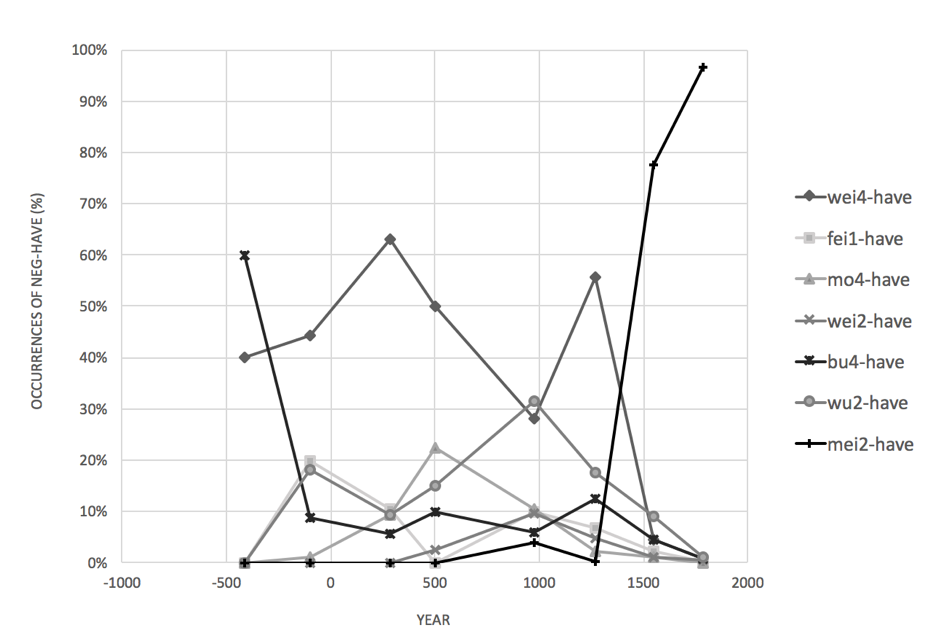
\includegraphics[height=.5\textheight]{figures/fig_lam1.png}
  \caption{Percentage of NEG+HAVE realisations in historical texts (version 1).}
  \label{fig:lam1}
\end{figure}

The x-axis in \figref{fig:lam1} represents the years, with 0 designating the year AD 1. The minus before some years replaces the abbreviation BC. Each line represents one form of realisation of \textsc{neg}+\textsc{have} and all of them have eight points, each of which marks the result from one of the eight texts selected for this study. The y-axis represents the proportion of each \textsc{neg}+\textsc{have} combination over the total number of \textsc{neg}+\textsc{have} occurrences in the text. For instance, 莫有 \textit{mò}-have has occurred ten times in the third text, \emph{Records of the Three Kingdoms} (AD 265–300), out of a total of 106 \textsc{neg}+\textsc{have} occurrences, hence the percentage shows 9.43\% at the third point of the line. In another text produced later in history, a fourth text, \emph{A New Account of the Tales of the World} (AD 420–581), which was produced later, only has nine occurrences of the form \textit{mò}-have, but as there were only 40 tokens of \textsc{neg}+\textsc{have} in this text, the percentage marked at the fourth point of the same line is 22.5\%. The prominent pattern in \figref{fig:lam1} is that many different \textsc{neg}+\textsc{have} combinations have been consistently attested across the eight texts, although the number of their occurrences were rather low. The forms \textit{wéi}-have, \textit{mò}-have, and \textit{fēi}-have serve as examples of this. There are four particular \textsc{neg}+\textsc{have} combinations that have displayed more substantial changes over time: \textit{wèi}-have (未有 \textit{wèi-yǒu}), \textit{bù}-have (不有 \textit{bù-yǒu}), \textit{wu2}-have (無有 \textit{wú-yǒu}), and \textit{mei2}-have (沒有 \textit{méi-yǒu}), with the latter being the focus of this analysis. For clarity, these results are repeated in \figref{fig:lam2} which uses the same design as \figref{fig:lam1}.

\begin{figure}
  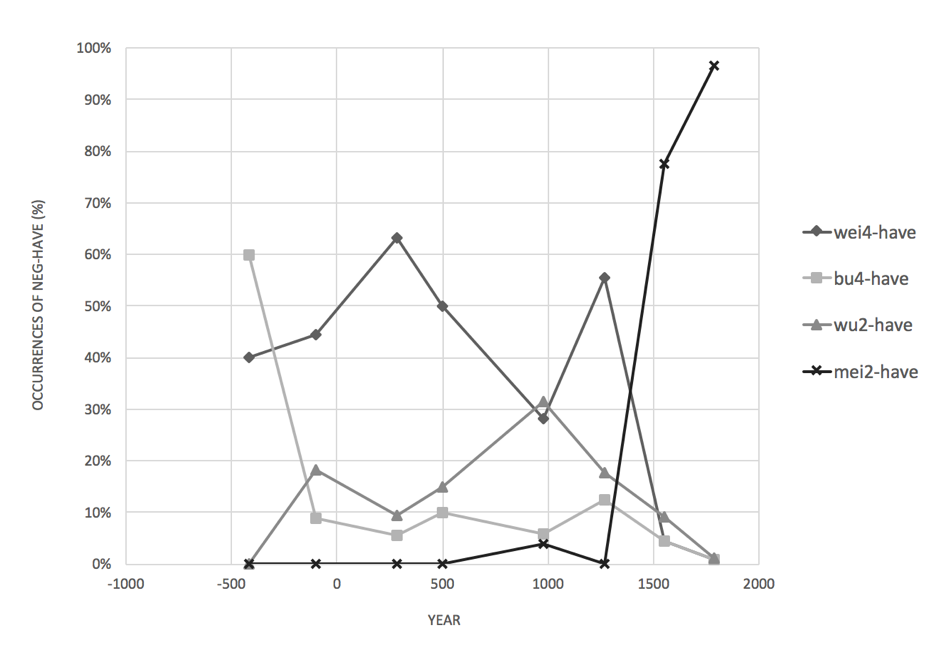
\includegraphics[height=.5\textheight]{figures/fig_lam2.png}
  \caption{Percentage of NEG+HAVE realisations in historical texts (version 2).}
  \label{fig:lam2}
\end{figure}

\figref{fig:lam2} reveals three important findings. Firstly, \textit{bù}-have is the earliest realisation of \textsc{neg}+\textsc{have} combination in \emph{The Analects} (BC 480–350), but appearances of this form diminished in approximately AD 1300. Secondly, \textit{wú}-have emerged as a competing form of \textsc{neg}+\textsc{have} against \textit{bù}-have, and its usage constantly increased until around AD 1300. The discovery that \textit{bù} and \textit{wú} have coexisted since the Old Chinese period concurs with the traditional understanding of the M-/P division of negation in Old Chinese (see \citealt{Hashimoto1985} and \citealt{Zhang2002} for more details). In brief, the issue of M-/P-negation division concerns the historical observation that Old Chinese had two groups of negators which were distinguishable by their initial consonant. One of these groups has an initial nasal, while the other has a plosive. The contemporary Chinese equivalent to this nasal-plosive (also referred to as the M-/P division) is arguably the North-South division of regional varieties. Evidence for this is the `not' negator. The Northern varieties have a plosive `not', such as the Beijing Mandarin \textit{bù}, while the Southern varieties have a nasal `not', such as the Hong Kong Cantonese \textit{m4} and the Gaozhou Cantonese \textit{mau5}; \tabref{tab:lam5} presents additional information on the regional M-/P-division (adapted from \citealt{Hashimoto1985} and \citealt{Zhang2002}).\footnote{The phonological representation in \tabref{tab:lam5} follows the IPA. The cities are arranged according to their geographical location from north to south, the labels N(orth) and S(outh) are determined by whether they are to the north or south of Chang Jiang (also known as the Yangtze River), which is the traditional means of defining the north-south divide in China.}

\begin{table}
  \begin{tabularx}{\textwidth}{L{1cm}XXX}
    \lsptoprule
    & & `not' & `not have'\\
     \midrule
N &{\cn 瀋陽}  Shenyang & pu & mei (iou)\\
N &{\cn 北京}  Beijing & pu & mei (iou)\\
N &{\cn 濟南}  Jinan & pu & mei (iou); mu (iou)\\
N &{\cn 西安}  Xian & pu & mo iou; m iou\\
N &{\cn 合肥}  Hefei & pəʔ & me; mɯ\\
S &{\cn 蘇州}  Suzhou & fəʔ & m pɤʔ\\
S &{\cn 南昌}  Nanchang & pət & mau iu\\
S &{\cn 長沙}  Changsha & pu & mau tɤ; mau\\
S &{\cn 溫州}  Wenzhou & fu & nau < m-\\
S &{\cn 福州}  Fuzhou & ŋ̩ < m̩ & mɔ\\
S &{\cn 廈門}  Xiamen & m̩ & bo < m-\\
S &{\cn 汕頭}  Shantou & m̩ & bo < m-\\
S &{\cn 梅縣}  Meixian & m̩ & mɔ\\
S &{\cn 廣州} Guangzhou & m̩ & mou\\
\lspbottomrule
\end{tabularx}
  \caption{The M-/P-division in the negator of regional varieties}
  \footnotemark
  \label{tab:lam5}
\end{table}

\footnotetext{The phonological representation in \tabref{tab:lam5} follows the IPA. The cities are arranged according to their
geographical location from north to south, the labels N(orth) and S(outh) are determined by whether they
are to the north or south of Chang Jiang (also known as the Yangtze River), which is the traditional means
of defining the north-south divide in China.}

\tabref{tab:lam5} shows that what is referred to as the M-/P-division may not be as clear cut as it seems, and that instead of a rigid line, this `division' should be conceived of as a continuum where gradual changes are evident, from the dominant M-form in the south to the non-nasal form in the north. A non-nasal, non-plosive F-form `not' has also emerged between these two zones, as attested in Suzhou and Wenzhou.

\citet{Zhang2002} suggests that the M-/P division of negation has crucial consequences in the sense that M-negators across the varieties of Chinese follow \citeauthor{Croft1991}'s NEC and associate closely with non-existence, whereas this is not the case for the P-negators. According to \citeauthor{Zhang2002}'s analysis, the Chinese negation system belonged to Type B\sim C in its earliest oracle bone records, where \textit{wú} acted as both the special form for the negative existential and a verbal negator in some contexts, but as \textit{wú} was not the only verbal negator, the system cannot be classified as Type C. In Later Old Chinese, the system might have evolved into Type A, where \textit{wú} requires the presence of the verb \textit{yǒu} `have' to express negative existence. By Middle Chinese, the [\textit{wú}-have DP] structure (that is, \textit{wú} negating the existential predication of \textit{yǒu} and its nominal complement) became more common and the use of \textit{wú} and other derived forms such as 毛 \textit{mau} prevailed particularly in the southern varieties. By the late Tang dynasty (ca. tenth century AD), the M-negators dominated the southern part of China, while the P-negators remained popular in the North. The key stages are summarised in \tabref{tab:lam6} below.


\begin{table}[]
	\caption{Historical development in expression of the negative existential}
	\label{tab:lam6}
	\begin{tabular}{lllll}
	\lsptoprule
	& \multicolumn{2}{l}{Old Chinese} & \multirow{2}{*}{Middle Chinese} & \multirow{2}{*}{Pre-Modern Chinese} \\
	& Early & Later &  &  \\ \midrule
   North & \multirow{2}{*}{\begin{tabular}[c]{@{}l@{}}\textbf{B$\sim$C}\\ m-negators\\ as NEG.EX\\ and verbal\\ negator\end{tabular}} & \multirow{2}{*}{\begin{tabular}[c]{@{}l@{}}\textbf{B$\sim$C}\\ \textit{wú*(have)}\\ as NEG EX\end{tabular}} & \begin{tabular}[c]{@{}l@{}}\textbf{A}\\ \textit{wu have DP}\end{tabular} & \begin{tabular}[c]{@{}l@{}}M- and P-negators\\ co-exist\end{tabular} \\ \cmidrule(r){1-1} \cmidrule(l){4-5} 
   South &  &  & \begin{tabular}[c]{@{}l@{}}\textbf{B}\\ \textit{mou (=wu)} and\\ other derived\\ forms emerged\end{tabular} & M-negators dominates \\ \lspbottomrule
	\end{tabular}
\end{table}



\citeauthor{Zhang2002} proposed that in southern varieties such as Cantonese and Hakka, their `not' negators were derived from their `not have' negators which were once the general negator (see also \citealt{Law2014} which suggested that the Hong Kong Cantonese \textit{mou5} `not.have' was the product of \textit{mou4} + \textit{jau5} `not + have'). Another standard negator could have been invented for the sake of keeping the negation of the existential distinct from the negation of normal verbs as suggested by \citet{Veselinova2016}. I will return to \citeauthor{Zhang2002}'s analysis of the Cantonese negators in §\ref{s:lam5}, but it is important to mention that \citeauthor{Zhang2002} has not explained how the Mandarin negation system evolved from the Old Chinese state to its present form, or in other words, how \textit{méiyǒu} emerged as the negative existential predicate and standard negator. It is significant that the sample texts featured in \figref{fig:lam2} have no recordings of \textit{méi}-have (or \textit{méiyǒu}) until AD 1300, and afterwards, \textit{méiyǒu} has become the predominant form to express the \textsc{neg}+\textsc{have}. The situation continues at present as well, as contemporary Mandarin has no other acceptable forms of \textsc{neg}+\textsc{have}. The emergence of \textit{méiyǒu} may seem rather sudden (\figref{fig:lam2}), but it is reasonable to postulate that this sudden appearance of \textit{méiyǒu} found in the texts only marked the beginning of the documentation of more colloquial speech and it is not the actual point where the strategy emerged. The late thirteenth century to the beginning of the fourteenth century marks the end of a long history of Han rule and the beginning of `foreign' rule – the Yuan dynasty (AD 1271–1368). This was a period when the Mongolians ruled the entire nation. The issue at hand is to determine how \textit{méiyǒu} became the predominant form for \textsc{neg}+\textsc{have}, and how that resulted in its development into a standard negator in present-day Mandarin varieties.



\subsection{Emergence of \textit{méi(yǒu)} as a negative existential and standard negator}\label{s:lam4-2}

Based on the historical texts (beyond the eight selected texts) in the \cite{chant} and Chinese Text Project, 沒 \textit{méi}/\textit{mò} first appeared during the Pre-Qin era where it had three related meanings: to sink or submerge, to die, and the end of something, as illustrated in examples (\ref{ex:lam18}), (\ref{ex:lam19}), and (\ref{ex:lam20}), respectively. It is important to note that although these three readings of 沒 \textit{méi}/\textit{mò}  are archaic, they continue to be found in present-day Chinese, such as, in Mandarin and Cantonese. When this lexical item is used to express its three meanings in Beijing and Taiwan Mandarin, its phonological realisation is \textit{mò} (\textit{mut6} in Hong Kong Cantonese). Whereas, when it functions as a standard negator, it is realised as \textit{méi}. This function is not found in Cantonese but if it were, the phonological form would still be \textit{mut6}. For ease of exposition, I follow the pronunciation in contemporary Mandarin when glossing the lexical uses of this word as \textit{mò} and its negation uses as \textit{méi} in the examples and in the text. An important point to note, however, is that in terms of sound change, \textit{méi} did not develop from \textit{mò} (\citealt[390]{Schuessler2007}).

\ea \textit{Mò} `to sink or submerge'  \label{ex:lam18}\\
  \ea {\cn 不臨深泉, 何以知\textbf{沒}溺之患} \label{ex:lam18a}\\
  	\gll bu lin shen quan, heyi zhi \textbf{mo}-ni-zhi huan\\
  	not come	 deep stream how know \textbf{submerge}-drown-gen danger\\ 
  	\glt `If one does not come close to a deep stream, how can one understands the danger of drowning?' ({\cn 《孔子家語》}\emph{Kongzi Jiayu} 206 BC–AD 220)
  \ex {\cn 可以步行水上不\textbf{沒} }\label{ex:lam18b}\\
  	\gll keyi buxing shui shang bu \textbf{mo}\\ 
  	can walk water above not \textbf{sink}\\
  	\glt `[He] can walk on water and won't sink.' ({\cn 《抱朴子》}\emph{Baopuzi} AD 300–343)
  \ex {\cn 日月出\textbf{沒}其中} \label{ex:lam18c}\\
	\gll ri yue chu \textbf{mo} qi zhong\\ 
	sun	moon	 out \textbf{sink} \textsc{pro} within\\ 
	\glt `The sun and moon appear there.' ({\cn 《藝文類聚》}\emph{Yiwen Leiju} AD 624)
\z \z 

The main verb of the subordinate clause that denotes the action of sinking in example (\ref{ex:lam18b}) is \textit{mò}. The following example, (\ref{ex:lam18c}), is a quote from a later text, \emph{Yiwen Leiju} – an encyclopedia compiled during the Tang dynasty (AD 624AD). This quote illustrates how the meaning `to sink/submerge' has been extended to non-human entities, such as the sun and the moon (for instance, the sunset is depicted as the sun sinking or submerging). Crucially, \textit{mò} appears with \textit{nì} `drown' in (\ref{ex:lam18a}) and together they mean that someone sank and drowned, which reflects the natural link between sinking and death: sinking or submerging leads to drowning, with results in death. 

Indeed, \textit{mò} also denotes `to be dead' in the examples below: 

\ea \textit{Mò} `to be dead'  \label{ex:lam19}\\
  \ea {\cn 父在, 觀其志; 父\textbf{沒}, 觀其行 \label{ex:lam19a}}\\
  	\gll fu zai, guan qi zhi; fu \textbf{mo}, guan qi xing\\
  	father live observe	his	will father	\textbf{die} observe his	conduct\\
  	\glt `While one's father lives, observe his aspiration; when one's father dies, observe his conduct.' ({\cn 《論語》}\emph{The Analects} BC 480–350)
  \ex {\cn 二親既\textbf{沒}, 所居齋寢} \label{ex:lam19b}\\
  	\gll er	qin	ji \textbf{mo}, suo ju zhai qin\\
  	two	parents	already	\textbf{die} \textsc{pro} dwell alone	sleep\\
  	\glt `With the death of the parents, [he] lived alone in [his] place (for mourning).' ({\cn 《顏氏家訓》}\emph{Yanshi Jiaxun} AD 420–581)
  \ex {\cn 生有顯功,\textbf{沒}有美名 }\label{ex:lam19c}\\
	\gll sheng you xian gong, \textbf{mo} you mei ming\\ 
	live have remarkable feat \textbf{dead} have	good name\\
	\glt `[He] had remarkable achievements when he lived, and a good name after he died.' ({\cn 《藝文類聚》}\emph{Yiwen Leiju} AD 624)
\z \z

Example (\ref{ex:lam19a}) is a clear case in point. The parallelism of the two sentences is deliberately used to highlight the contrast in content. The first clause in the first sentence is `when father lives', and in the second sentence, the first clause expresses the opposite, `when father dies', and the meaning of `to die' is encoded by \textit{mò}. At a glance, example (\ref{ex:lam19c}) appears to present a case of \textit{mò yǒu} (also known as \textit{méiyǒu}), where \textit{yǒu} is the possessive predicate and 沒 \textit{méi}/\textit{mò} is the negator, but this would be a misinterpretation. Similar to example (\ref{ex:lam19a}), this sentence contains two clauses with parallel structure, expressing a contrastive meaning: the first clause states that the person in question (although pro-dropped) attains remarkable achievements when he lives, and the second clause contrasts that by stating what he possesses when he dies. In both clauses, the verb \textit{yǒu} `have' means `to possess/own', and 沒 \textit{méi}/\textit{mò} in the second clause means `dead' (hence it is glossed as \textit{mò}, not \textit{méi}), the opposite of \textit{shēng} `live' in the first clause. 

The third meaning of \textit{mò} is `the end of something', and this meaning, which existed at the same time as the other two, is an extension of the notion of death which we have seen in example (\ref{ex:lam19}). Just as the meaning of `to sink/submerge' has been metaphorically extended to the sun (as in, the sunset) the concept of death being the end of the life can likewise be extended to non-human entities. The concept of death can be `the end' in general and this is illustrated by the examples in (\ref{ex:lam20}) below. 

\ea \textit{Mò} `the end of something'  \label{ex:lam20}\\
  \ea {\cn 於夏十月, 火既\textbf{沒}矣} \label{ex:lam20a}\\
  	\gll yu xia shi yue, huo ji	\textbf{mo} yi\\
  	in	Summer	tenth	month fire already \textbf{exhaust} \textsc{prt}\\
  	\glt `In Summer, October, when the fire has died down' ({\cn 《孔子家語》}\emph{Kongzi Jiayu} 206BC–AD 220)
  \ex {\cn 恐\textbf{沒}世不復見如此人} \label{ex:lam20b}\\
  	\gll kong \textbf{mo} shi bu fu jian ruci ren\\
  	fear \textbf{end} world not again	see	such person\\
  	\glt `Fear that it won't be possible to find such person till end of the world' ({\cn 《世說新語》}\tablevspace\emph{A New Account of the Tales of the World} AD 420–581)
  \ex {\cn 立言不\textbf{沒}} \label{ex:lam20c}\\
	\gll li yan bu \textbf{mo}\\
	establish word not \textbf{end/extinguish}\\
	\glt `The words [one] established do not perish.' ({\cn 《藝文類聚》}\emph{Yiwen Leiju} AD 624)
\z \z

When \textit{mò} denotes `the end of something', it can be used as a verb (such as `to end') or an adjective (such as `final'). The former is illustrated by examples (\ref{ex:lam20a}) and (\ref{ex:lam20c}), and the latter by (\ref{ex:lam20b}). Once the meaning of \textit{mò} has been semantically `stretched' to mean `death,' or even `the end,' both of which practically indicate that the entity in question ceases to exist, \textit{mò} has become a natural candidate to express non-existence in general. Indeed, by the late thirteenth century, the negative existential function of 沒 \textit{méi} emerged (\ref{ex:lam21}), as did its use as a verbal negator (\ref{ex:lam22}). \citet{Xu2003} presents an alternative position that the emergence of \textit{méi} could be phonologically-driven. According to \citeauthor{Xu2003}, sound change occurred approximately during the tenth century AD making \textit{wú} (\textit{mou4} in Hong Kong Cantonese, which resembles the Middle Chinese realisation more closely) and \textit{mò} almost indistinguishable phonetically. As a result, by the Song dynasty (AD 960–1279), \textit{mò} and \textit{wù} tended to be used interchangeably, and by around the fifteenth century, \textit{méi}/\textit{mò} has completely replaced \textit{wú} as the negative existential (see \citealt{PanW2002} and \citealt{Xu2003}). In fact, the semantic bleaching and sound change accounts fit rather well in terms of timing and the empirical evidence, and it is likely that both factors contributed and motivated the rise of \textit{méi}/\textit{mò} as the new negative existential predicate. This special form for the negative existential later developed into a standard negator in contemporary Mandarin varieties, confirming the NEC prediction. \citet[376--377, 517--518]{Schuessler2007} mentions that two possible pathways have been proposed. On the one hand, \citet[126]{Norman1988} suggests that \textit{méi} (which was pronounced muət in Middle Chinese) could be a variant of
{\cn 勿} \textit{wú} or
{\cn 未} \textit{wèi}, and that this variant was later fused with or influences by \textit{yǒu} `have'. On the other hand, \citet[121]{Pulleyblank1973} proposes that the etymology of `not have' originated from `submerge'. It began from the reconstructed form *\textit{ma}, continued to
{\cn 末} \textit{mò} `the end of something' and to
{\cn 亡 \textit{wáng}} (\textit{mong4} in Hong Kong Cantonese) `to die or be dead', then to
{\cn 無} \textit{wú} (Hong Kong Cantonese \textit{mou4}) `not or nothing' or
{\cn 莫} \textit{mò} `not or don't', and finally to
{\cn 沒} \textit{mò}/\textit{méi} as `not have'. A thorough examination of which of the two factors played a more significant role in the historical development would, however, go beyond the scope of the present study.


\ea \textit{Méi} as a negative existential \label{ex:lam21}\\
  \ea {\cn 一向都\textbf{沒}分別} \label{ex:lam21a}\\
  	\gll yixiang dou \textbf{mei} fenbie\\
  	along all \textbf{\textsc{mei}} difference\\
  	\glt `There's no difference all along.' ({\cn 《朱子語類》}\emph{Zhuzi Yulei} AD 1270)
  \ex {\cn 將船撐至\textbf{沒}人煙處} \label{ex:lam21b}\\
  	\gll jiang chuan cheng zhi \textbf{mei} renyan chu\\
  	make boat punt till \textbf{\textsc{mei}} people.smoke place\\
  	\glt `[He] punted the boat to a place without people.' ({\cn 《西遊記》}\emph{Journey to the West} AD 1520–1580)
  \ex {\cn \textbf{沒}人照顧} \label{ex:lam21c}\\
	\gll \textbf{mei} ren zhaogu\\
	\textbf{\textsc{mei}}	people	take.care\\
	\glt `There is no one to look after him.' or `He has no one to look after him.' ({\cn 《儒林外史》}\emph{The Scholars} AD 1750)
\z \z

\ea \textit{Méi} as verbal negator: {\cn 都\textbf{沒}理會了} \label{ex:lam22}\\
  \gll dou \textbf{mei} lihui le\\
  all \textbf{\textsc{mei}} take.notice le\\
  \glt `[they] all didn't take notice.' ({\cn 《朱子語類》}\emph{Zhuzi Yulei} AD 1270)
\z

The negative existential predication and general verbal negation functions of \textit{méi} emerged almost simultaneously. This is made evident by a text from the Song dynasty, \emph{Zhuzi Yulei}, which is a collection of philosophical dialogues between \emph{Zhuzi} and his students compiled in AD 1270. Example (\ref{ex:lam21a}) is extracted from this same text and is an instance of \textit{méi} denoting the non-existence of an entity, \textit{fēnbié} `difference', although the locative reference that we have seen in the Old Chinese examples of \textit{yǒu} `have' (\ref{ex:lam15a}–\ref{ex:lam15b}) is absent. Example (\ref{ex:lam22}), on the other hand, shows \textit{méi} as a verbal negator because it denies that the event of `taking notice' has occurred. It is important to note that the negative existential predicate and verbal negator \textit{méiyǒu} did not occur in the texts before the fourteenth century. In other words, the functions of \textit{méi} as the negative existential predicate and as the verbal negator long predate the appearance of \textit{méiyǒu}. It was not until the Ming dynasty (AD 1368–1644) that the \textit{méi-yǒu} `not-have' combination first appeared as a negative existential expression as shown in (\ref{ex:lam23}). By the eighteenth century, \textit{méiyŏu} `not have' combination began to function as a verbal negator. The first documented case of this was found in Dream of the Red Chamber (AD 1748), which is featured in example (\ref{ex:lam24}). 


\ea \textit{Méiyǒu} as a negative existential \label{ex:lam23}\\
  \ea {\cn 連宿處也\textbf{沒}有了} \label{ex:lam23a}\\
  	\gll lian shu chu ye [\textbf{mei} you] le\\ 
  	even sleep place also [\textbf{\textsc{mei}} have] \textsc{le}\\
  	\glt `There isn't even a place to stay now.' or `[We] don't have a place to stay.' ({\cn 《西遊記》}\emph{Journey to the West} AD1520–1580)
  \ex{\cn  此處並\textbf{沒}有什麼蘭麝、明月、洲渚之類 }\label{ex:lam23b}\\
  	\gll ci chu bing [\textbf{mei} you] shenme lanshe mingyue zhou chu zhi lei\\
  	this	 place really [\textbf{\textsc{mei}} have] what fragrant.herbs bright.moon is let that kind\\ 
  	\glt `There isn't herbs, moon, islet or the likes [elements for poetry] here.' ({\cn 《紅樓夢》}\emph{Dream of the Red Chamber} AD 1748)
\z \z


\ea \textit{Méiyǒu} as verbal negator:{\cn  還\textbf{沒有}走到跟前} \label{ex:lam24}\\
  \gll hai [\textbf{mei-you} zou-dao] genqian\\
  still [\textbf{not-have} walk-\textsc{cpl}] in.front\\
  \glt `still have not walked to the front.' ({\cn 《紅樓夢》}\emph{Dream of the Red Chamber} AD 1748)
\z


A world-renowned novel from the Ming dynasty, \emph{Journey to the West}, contained many tokens of \textit{méiyǒu} that expressed negative existence such as the one in example (\ref{ex:lam23a}). But example (\ref{ex:lam23a}) also reveals the ambiguity involved in the expression. As subject pro-drop has been very common in Chinese, instances such as (\ref{ex:lam23a}) can be interpreted as `someone does not even have a place to stay' or that `this place or there does not even have a place for people to stay'. If it is the former (when the subject is a human), then (\ref{ex:lam23a}) is a possessive structure and \textit{méiyǒu} means `not possess', but if the latter is true (when the sentence has a locative subject), then it is an existential construction, and \textit{méiyǒu} means `not exist', as it does in the sentence in (\ref{ex:lam23b}). The ambiguity is significant to the development of \textit{méiyǒu} from a negative existential predicate to a verbal negator (and a standard negator). As \textit{yǒu} `have' can be an existential predicate and a possessive predicate, it might have provided a stepping stone for \textit{méi} to evolve from a negative existential predicate to a standard negator. Indeed, the verb \textit{yǒu} `have' has been polysemous in expressing existence and possession ever since the Old Chinese period; its existential sense has been discussed in \sectref{s:lam4-1} and the examples below illustrate \textit{yǒu} `have' as a possessive predicate.


\ea `Have' as possessive predicate \label{ex:lam25}\\
  \ea{\cn  秦王\textbf{有}虎狼之心 }\label{ex:lam25a}\\
  	\gll Qin	wang \textbf{you} hu lang zhi xin\\
  	Qin	emperor	\textbf{have} tiger wolf \textsc{gen} heart\\
  	\glt `The Emperor of Qin is full of ambition and calculation.' (lit. `The Emperor of Qin has a heart like the tiger or wolf.') ({\cn《史記·項羽本紀》}\emph{Shiji} 109–91 BC)
  \ex{\cn  庾子躬\textbf{有}廢疾,甚知名} \label{ex:lam25b}\\
  	\gll Yu Zigong \textbf{you} feiji, shen zhiming\\
  	Yu Zigong \textbf{have} disability quite	well-known\\
  	\glt `Yu Zigong has physical disability which is quite well-known.' ({\cn《世說新語》}\emph{A New Account of the Tales of the World} AD 420–581)
\z \z

(\ref{ex:lam25a}) is an example of Old Chinese, where \textit{yǒu} `have' is the main verb that predicates over the nominal complement, \textit{hǔ láng zhī xīn} `ambition' (literally, `the heart of the tiger or wolf'), and the subject \textit{Qín wáng}, `King of Qin', is the possessor. Likewise, in (\ref{ex:lam25b}), the subject (\emph{Yǔ Zǐgōng}) possesses a physical disability, and the verb \textit{yǒu} denotes `to possess'. 

To summarise, the development of Chinese negation began with a highly diverse situation where more than ten negative markers actively existed in the language, and among those negative markers, at least three were productive strategies to express negative existence:

% example 26
%\bigskip
%Old Chinese negative existential expressions
%\begin{enumerate}
%	\item \textit{wú} can stand alone as a special form of the negative existential (\citealt{Zhang2002}), 
%	\item \textit{bù} can negate the existential predicate \textit{yǒu} `have' to express negative existence, and 
%	\item \textit{wú} can combine with the existential predicate \textit{yǒu} `have' to express negative existence.
%\end{enumerate}

% example 26 turned into a table  
\begin{table}
  \begin{tabularx}{\textwidth}{lQ}
    \lsptoprule
     %\midrule
\textit{wú} & can stand alone as a special form of the negative existential (\citealt{Zhang2002})\\
\textit{bù} & can negate the existential predicate \textit{yǒu} `have' to express negative existence\\ 
\textit{wú} & can combine with the existential predicate \textit{yǒu} `have' to express negative existence\\
\lspbottomrule
\end{tabularx}
  \caption{Old Chinese negative existential expressions}
  \label{ex:lam26}
\end{table}


Following \citeauthor{Croft1991}'s NEC classification, Old Chinese displayed signs of the Type A system with the second strategy (\textit{bù-yǒu}), the Type B system with the first strategy (\textit{wú}), as well as the B\sim C (or even C\sim A) system with the third strategy (\textit{wú-yǒu}). In other words, because \textit{wú} was only one of the Chinese verbal negators, it should be considered as Type B\sim C, but its presence with the existential predicate in negative existential contexts resembles the C\sim A system, hence the ambiguity. These strategies for the negative existential continued to be competing alternatives in historical records until a `novel' form, \textit{méi}, emerged in the late thirteenth century AD. That form developed through a series of semantic extensions and bleaching from `sink' to `dead', and then became a form to express non-existence and general verbal negation. Therefore, \textit{méi} initially was a special form for the negative existential and also basically a verbal negator (in other words, Type B\sim C). 

While \textit{méi} later became compatible with the existential predicate \textit{yǒu} `have' in negative existential contexts, \textit{méi-yǒu}, similar to \textit{wú-yǒu}, can be ambiguously interpreted as a sign of a B\sim C or C\sim A system. The sign of Type B\sim C is that \textit{méi} and \textit{bù} co-exist as standard negators in contemporary Mandarin, and the sign of Type C\sim A is that \textit{méi} itself is both a negative existential predicate and a verbal negator. Its compatibility with \textit{yǒu} `have' could indicate that the system is moving on to the compositional Type A. The historical development sketched in this section has important implications for the analysis of contemporary Mandarin negation. Firstly, the fact that \textit{méi} predates \textit{méiyǒu} in being a negative existential predicate and a verbal negator indicates that \textit{méi} cannot be interpreted as a contracted form of \textit{méiyǒu}. The optional presence of \textit{yǒu} in present-day Mandarin varieties is not simply a matter of phonological fusion or reduction in the fact that \textit{yǒu} can appear with \textit{méi} in negative existential contexts and standard negation indicates that the existential content of \textit{méi} may be bleached. This results in the presence of \textit{yǒu} being acceptable and not semantically redundant; and its optionality shows that the semantic bleaching remains underway. Secondly, the development of \textit{méi} from a negative existential predicate to verbal negation might explain why \textit{yǒu} must be negated by \textit{méi}, while other verbs can be negated by either \textit{méi} or \textit{bù}. The connection between \textit{méi} and \textit{yǒu} rests in their semantic connection, that is, existence. The next section will examine the negation system of two Cantonese varieties (Hong Kong and Gaozhou Cantonese) from the perspective of the NEC. The result will not only highlight the cross-linguistic similarities and differences, but will also account for the ambiguous statuses of \textit{wú-yǒu} and \textit{méi-yǒu}. 



\section{Variation within Chinese}\label{s:lam5}

The connection that \citeauthor{Croft1991} identified between the NEC and Mandarin Chinese also exists in the Cantonese varieties of Chinese. The verb `to have' is generally used as the existential predicate in Chinese varieties, but it has varying phonological forms in different varieties. Thus, the verb `to have' is \textit{yǒu} in Mainland and Taiwan Mandarin and \textit{jau5} in Hong Kong and Gaozhou Cantonese. The existential constructions in the Cantonese varieties are illustrated in the examples below: 


\ea Hong Kong Cantonese (Yue Chinese, Sinitic) \label{ex:lam27}\\
  \ea {\cn 課室度\textbf{有}鉛筆 }\label{ex:lam27a}\\
  	\gll fosat	dou	\textbf{jau} jyunbat\\
  	classroom place	\textbf{have} pencil\\
  	\glt `There are pencils in the classroom.'
  \ex{\cn  課室度\textbf{唔有}鉛筆 }\label{ex:lam27b}\\
  	\gll *fosat	dou	\textbf{m} \textbf{jau} jyunbat\\
  	classroom place	\textbf{not} \textbf{have} pencil\\
  	\glt `There aren't pencils in the classroom.'
  \ex{\cn  課室度冇(*\textbf{有})鉛筆 }\label{ex:lam27c}\\
  	\gll fosat	dou	\textbf{mou} (*\textbf{jau}) jyunbat\\
  	classroom	place	\textbf{not.have}	\textbf{have}	pencil\\
  	\glt `There aren't pencils in the classroom.'
\z \z
 
\ea Gaozhou Cantonese (Gaoyang Yue Chinese, Sinitic) \label{ex:lam28}\\
  \ea{\cn  課室具}\footnote{The character is merely an approximation for the phonetic realisation of \textit{gui3} because Cantonese generally lacks systematic orthography.}{\cn \textbf{有}鉛筆} \label{ex:lam28a}\\
  	\gll fosat gui \textbf{jau} jinbat\\	
  	classroom that.place \textbf{have} pencil\\
  	\glt `There are pencils in the classroom.'
  \ex {\cn 課室具\textbf{茅有}鉛筆} \label{ex:lam28b}\\
  	\gll fosat gui \textbf{mau} (\textbf{jau}) jinbat\\
  	classroom that.place \textbf{not} \textbf{have} pencil\\
  	\glt `There aren't pencils in the classroom.'
\z \z

Examples (\ref{ex:lam27a}) and (\ref{ex:lam28a}) above contain the existential construction in Hong Kong Cantonese and Gaozhou Cantonese in an affirmative context, respectively. Both varieties use the verb \textit{jau5} `to have' to express the existence of the entity denoted by its complement, which is a pencil, with reference to a location, such as a classroom. This affirmative structure is equivalent to the one found in the Mandarin varieties (\ref{ex:lam13}). However, the negative sentences in examples (\ref{ex:lam27b}) and (\ref{ex:lam27c}) as well as in example (\ref{ex:lam28b}) are notably different. Firstly, Hong Kong Cantonese has two standard negators, \textit{m4} `not' and \textit{mou5} `not.have'. These largely resemble \textit{bù} and \textit{méi(yǒu)} in Mandarin, but the Mandarin \textit{yǒu} `have' has the option to follow \textit{méi} but \textit{jau5} in Hong Kong Cantonese cannot co-occur with \textit{mou5}. Examples (\ref{ex:lam27b}) and (\ref{ex:lam27c}) reveal that the only legitimate negator in Hong Kong Cantonese negative existential constructions is \textit{mou5}, but even there the presence of the existential predicate \textit{jau5} is strictly forbidden. In addition, Gaozhou Cantonese differs from the other three varieties in having only one standard negator \textit{mau5} `not'. Thus, the counterpart of Gaozhou Cantonese in example (28b) resembles the Mandarin structure except that the negator \textit{mau5} is the only standard negator in the variety. In terms of classifying the Cantonese varieties into the NEC types, as the Hong Kong Cantonese \textit{mou5} `not.have' can express negative existence on its own, it can be regarded as a special form of negative existential, which means that Hong Kong Cantonese would be categorised at least as Type B. Hong Kong Cantonese \textit{mou5} `not.have' resembles Beijing and Taiwan Mandarin in that it can also be used as a standard negator even though this usage is subject to some restrictions, as shown in \tabref{tab:lam7}\footnote{To recap, `bare negatives' refer to the negative form of bare sentences with no overt aspect-marking or any type of adverbial modification.} as well as in example (\ref{ex:lam29}), which involves a non-psych stative predicate. Therefore, Hong Kong Cantonese should be Type B\sim C, which is the same classification as the Mandarin varieties.

\begin{table}
  \begin{tabularx}{\textwidth}{L{2.8cm}XX}
    \lsptoprule
    & Hong Kong & Cantonese\\
    & \textit{m4} & \textit{mou5}\\
    & `not' & `not.have'\\
     \midrule
State [+psych] & \ding{51} 4.6 & ?4.2\\
State [-psych] & \ding{51} 4.6 & ??2.6\\
Activity & \ding{51} 4.6 & \ding{51} 4.7\\
Accomplishment & ?4.2 & \ding{51} 4.5\\
Achievement & ??2.4 & \ding{51} 4.7\\
Semelfactive & ?4.3 & \ding{51} 5.0\\
\lspbottomrule
\end{tabularx}
  \caption{Bare negatives in Hong Kong Cantonese}
  \label{tab:lam7}
\end{table}

\ea Negation and a non-psych state:  {\cn 我 (唔/\textbf{冇}) 知道呢件事} \label{ex:lam29}\\
	\gll ngo (m/??\textbf{mou}) zidou li	gin	si\\
	I not/\textbf{not-have} know this \textsc{cl} event\\
	\glt Intended: `I do not know about this event.' `I did not know about this event.'
\z

From the perspective of \citeauthor{Croft1991}'s NEC, the three Chinese varieties that have two standard negators (`not' and `not have'), namely, Beijing Mandarin, Taiwan Mandarin, and Hong Kong Cantonese, all represent Type B\sim C. This means that they have a special form for the expression of the negative existential, `not have'. Gaozhou Cantonese is different from the four other Chinese varieties examined in this study because it only has one standard negator, \textit{mau5}. Example (\ref{ex:lam30}) presents the standard negation in Gaozhou Cantonese, where \textit{mau5} occurs in a preverbal position after the subject, similar to the other varieties. The acceptability of \textit{mau5} with various situation types is illustrated in \tabref{tab:lam8}.

\ea {\cn  我\textbf{茅}寫己封信 \label{ex:lam30}}\\
	\gll ngo \textbf{mau} se gei fung seon\\
	I \textbf{not} write this \textsc{cl} letter\\
	\glt `I don't write this letter.'
\z

\begin{table}
	\begin{tabular}{@{}ll@{}}
    \lsptoprule
    & Gaozhou Cantonese\\
    & \textit{mau5}\\
    & `not'\\
     \midrule
State [+psych] & \ding{51} 4.6\\
State [–psych] & \ding{51} 4.7\\
Activity & \ding{51} 4.6\\
Accomplishment & \ding{51} 4.5\\
Achievement & ?3.9\\
Semelfactive & \ding{51} 4.6\\
\lspbottomrule
\end{tabular}
  \caption{Bare negatives in Gaozhou Cantonese}
  \label{tab:lam8}
\end{table}

I argue that standard negation in Gaozhou Cantonese is an example of Type C\sim A in the NEC. Gaozhou Cantonese apparently lacks a special form for the negative existential, but at the same time, the presence of the existential predicate \textit{jau5} `have' is optional in negative existential contexts. This indicates that \textit{mau5} can alone express negative existence and could be developing into a special form for the negative existential. Hence, it is possible to assume that Gaozhou Cantonese is Type A\sim B. However, according to \citet{Zhang2002}, while \textit{wù} declined in use in the North during the Middle Chinese period, it became the predominant form for negative existence in the South and many phonologically derived forms emerged in the southern varieties. \citeauthor{Zhang2002} thus proposes that the M-negators could be the result of combining \textit{wú} – once a standard negator developed from a negative existential – and the existential predicate \textit{yǒu} (in Cantonese, \textit{mou4} and \textit{jau5}). \citeauthor{Zhang2002} cites a great number of Cantonese varieties as examples of this historical development, including, \textit{mou5} in standard Cantonese (Hong Kong Cantonese included) and \textit{mau5} in Xinyi Cantonese. This latter example is crucial precisely because (i) Gaozhou, Xinyi, and Huazhou are the three county-level cities within Maoming, the southwestern county in Guangdong Province, and (ii) the negator, \textit{mau5}, in the Xinyi variety is identical to that in Gaozhou Cantonese. 

As far as Hong Kong Cantonese is concerned, \citeauthor{Zhang2002}'s discovery has been supported by \citet{Law2014} where the phonological process involved is suggested to be as follows: %\todo{Had to redraw the figure}

\begin{figure}
	\caption{Hong Kong Cantonese (Yue Chinese, Sinitic): \textit{mou5 < mou4 + jau5}}
	\label{ex:lam31}
% 	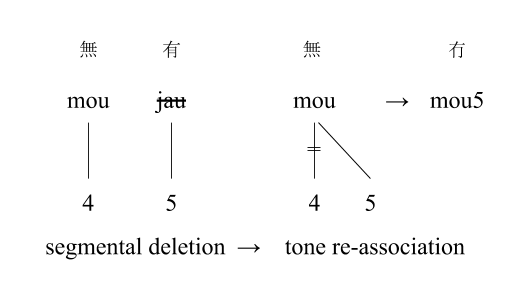
\includegraphics[width=0.75\textwidth]{figures/lam_ex31.png}
	\begin{forest}
	  [{}, phantom
	  [{{\cn 無}\\mou}      [4]]
	  [{{\cn 有}\\\st{jau}} [5]]
	  [~,phantom, no edge]
	  [{{\cn 無}\\mou}, name=mou [4, name=four]]
	  [{~\\~}                 [5,no edge, name=five]]
	  [{{\cn ~~~冇}\\\textrightarrow ~~ mou5}]
	  ]
	  \draw (five)--(mou.south);
          \node[above = 0mm of four]{=};
          \node[below = 0mm of four,xshift=-7mm]{segmental deletion \textrightarrow{} tone re-association};
	\end{forest}

\end{figure}

\citeauthor{Law2014} suggests that the marking of \textit{mou5} involved two processes: first, the segmental information in the existential predicate \textit{jau5} is deleted, then its tone (tone 5, the low-rising tone) is re-associated to the left, and replaced the original tone 4 of \textit{mou4}. The result is \textit{mou5}. Therefore, according \citeauthor{Law2014}, wherever \textit{mou5} appears, \textit{jau5} is also present in the structure but phonologically silent (see \citealt{Yue2001} for an alternative account which argues that \textit{mou5} is a product of \textit{m4} + \textit{jau5}; \textit{m} provides the initial consonant and \textit{jau5} provides the tone, and the vowel is influenced by the consonant). \citeauthor{Law2014}'s (\citeyear{Law2014}) analysis is supported by the reconstruction results in \citet{Norman1988} and \citet{Schuessler2007}. \citet[213]{Norman1988} notes that many M-negators in Chinese southern dialects are developed from {\cn 無} \textit{wù} and new negators are formed by the fusion of \textit{wù} and \textit{yǒu} (Hong Kong Cantonese \textit{mou4} and \textit{jau5} > \textit{mou5}). \citet[518--519]{Schuessler2007} further suggests that \textit{wù} developed to express negative existence or the meaning of `not have' in general (including negative possessive) during the Western Zhou period (1027–771 BC), and it later replaced all other forms with similar functions. Hence, {\cn 無} \textit{wù} is most probably the source of the negative existential and standard negator \textit{mou5} in contemporary Hong Kong Cantonese.

If \citeauthor{Law2014}'s (\citeyear{Law2014}) phonological analysis is well-founded and \citeauthor{Zhang2002}'s observation on Xinyi Cantonese \textit{mau5} is also applicable to Gaozhou Cantonese, they would carry two important implications. Firstly, the Gaozhou Cantonese \textit{mau5} is also a standard negator that has developed from the negative existential, similar to the other three varieties – \textit{méi(yǒu)} in Beijing and Taiwan Mandarin, and \textit{mou5} in Hong Kong Cantonese. In that case, Gaozhou Cantonese should not belong to Type A\sim B, but is a typical example of Type C\sim A. As \textit{mau5} alone can express negative existence, and acknowledging \citeauthor{Zhang2002}'s account that \textit{mau5} is derived from \textit{mou4} + \textit{jau5} `not [=not.have] + have',  \textit{mau5} itself is an example of a special form of the negative existential that has developed into a verbal negator. Indeed, the Gaozhou Cantonese data support this account: in terms of negation-viewpoint compatibility, \textit{mau5} resembles \textit{méi(yǒu)} and \textit{mou5} in being able to appear with the experiential viewpoint \textit{gwo3}. This would be unexpected if \textit{mau5} `not' should be patterned with the `not' negator of the other varieties, such as \textit{bù} and \textit{m4}. The major difference between Gaozhou Cantonese and the other three Chinese varieties is that this derived verbal negator is not only a standard negator but also the general negator in the variety. Once the existential predicate \textit{jau5} can once again appear with this derived negator (such as \textit{mau5}) in negative existential contexts, it would indicate that the negation system in Gaozhou Cantonese has moved to a full cycle, that is, C\sim A; this is indeed the case as seen in example (\ref{ex:lam28b}). The second point concerns the difference between \textit{méi(yǒu)} in the Mandarin varieties and \textit{mou5} in Hong Kong Cantonese. As classified above, Hong Kong Cantonese and the Mandarin varieties all belong to Type B\sim C, but unlike its Mandarin counterpart, \textit{mou5} cannot occur with \textit{jau5} as illustrated in (\ref{ex:lam27c}). This restriction not only applies to negative existential structures (such as when \textit{jau5} is an existential predicate), but occurs across the board – whenever \textit{mou5} is present \textit{jau5} must not, as shown in (\ref{ex:lam32}): 

\ea Hong Kong Cantonese (Yue Chinese, Sinitic) \textit{jau5} `have' \label{ex:lam32}\\
  \ea Existential negation: {\cn 課室度冇(*\textbf{有})鉛筆} \label{ex:lam32a}\\
  	\gll fosat dou \textbf{mou} (*\textbf{jau}) jyunbat\\
  	classroom	place	\textbf{not.have}	\textbf{have}	pencil\\
  	\glt `There aren't pencils in the classroom.'
  \ex Possessive negation: {\cn 我冇(*\textbf{有})鉛筆} \label{ex:lam32b}\\
  	\gll ngo	 \textbf{mou}	 (*\textbf{jau}) jyunbat\\
  	I \textbf{not} \textbf{have} pencil\\
  	\glt `I do not have/own pencils.'
  \ex Standard negation: {\cn 我冇(*\textbf{有})知道呢件事} \label{ex:lam32c}\\
  	\gll ngo	 \textbf{mou} (*\textbf{jau}) zidou li gin si\\
  	I \textbf{not.have} \textbf{have} know this	\textsc{cl}	event\\
  	\glt `I did not know about this event.'
\z \z

This would be expected if we follow the phonological account proposed by \citeauthor{Law2014}. The process applies indiscriminately to all syntactic structures precisely because \textit{jau5} is phonologically merged with \textit{mou4}. The Mandarin \textit{méi}, on the other hand, did not undergo the same phonological fusion process. \textit{Méi} developed into a negative existential predicate in Mandarin through a series of semantic change. These were from `to sink/submerge' which leads to the natural result of drowning and death (hence `to be dead') and later extended to mean `the end of something' which could develop from the idea of death being the end of life, the meaning of `end of something' or `something being extinguished or perished' can easily develop into the idea of non-existence, i.e. negative existence. \cite{Veselinova2013} identified three major sources in her typological study of negative existentials and these are summarised in \tabref{tab:lam9} (adapted from \citealt[Table 7]{Veselinova2013}):

\begin{table}
  \begin{tabularx}{\textwidth}{llY}
    \lsptoprule
    \multicolumn{2}{l}{Sources} & Number of languages\\
     \midrule
(i)	& Univerbation of standard negator and another word & 17 (27.0\%)\\
(ii) & Lexical item with a negative content & 25 (39.7\%)\\
(iii) & Formally identical with SN (origin unknown) & 21 (33.3\%)\\
\lspbottomrule
\end{tabularx}
  \caption{Summary of the origins of negative existentials}
  \label{tab:lam9}
\end{table}

Following \cite{Veselinova2013}, the Old Chinese \textit{wù} and the present-day Mandarin \textit{méi} are examples of the second source of negative existentials because they are lexical items with a negative content – \textit{wù} means `absent' and \textit{méi}/\textit{mò} can mean `dead', and both are common lexical sources for the negative existential in her typological study.\footnote{\cite{Veselinova2013} mentioned several common lexical origins for negative existential predicates: `lack', `absent', `there is not', `empty', and `dead'.} 
In contrast, the evolution of \textit{mou5} and \textit{mau5} in the two Cantonese varieties belong to source (i) where the negative existential was derived from the former standard negator \textit{mou4} (\textit{wú} in Mandarin) and the existential predicate \textit{jau5} `have'. The fact that \textit{méi} never contained a `have' element made it possible to appear with the existential predicate \textit{yǒu}. By comparison, since \textit{mou5} itself has evolved from \textit{mou4}-\textit{jau5}, co-occurrences of \textit{mou5} and \textit{jau5} in present-day Hong Kong Cantonese are blocked due to their structural clash and semantic redundancy. Comparing between the two Cantonese varieties, the possible though optional appearance of \textit{jau5} with \textit{mau5} for negative existence and negative possession indicates that the semantics of \textit{mau5} has been further bleached to the extent that its original meaning as a negative existential has been considerably weakened, whereas the sense of negative existence remains prominent in the \textit{mou5} of Hong Kong Cantonese.



\section{Conclusion}\label{s:lam6}

To summarise, this paper has based its arguments on historical evidence (from Old Chinese to Modern Mandarin and Cantonese) that \citeauthor{Croft1991}'s (\citeyear{Croft1991}) Negative Existential Cycle, which postulates the connection between negation and the existential predicate as a source for the evolution of general verbal negators, is indeed attested in Chinese history and in various Chinese varieties to date. Thus, according to the NEC classification, Beijing and Taiwan Mandarin as well as Hong Kong Cantonese belong to the transition Type B\sim C where \textit{méi} and \textit{mou5}, respectively, are special forms of the negative existential which have extended their use to general verbal negation but have not been generalised to the whole grammatical system; \textit{méi} and \textit{mou5} co-exist with \textit{bù} and \textit{m4} as standard negators in Mandarin and Hong Kong Cantonese, respectively. Gaozhou Cantonese, unlike the others, has a general negator \textit{mau5}, which this paper suggests, following \cite{Zhang2002} and \cite{Law2014}, to have derived from \textit{mou4} (once a special form for the negative existential) and the existential predicate \textit{jau5}. Since Gaozhou Cantonese allows the existential predicate \textit{jau5} `have' to optionally appear with \textit{mau5} even in negative existential contexts, I argue that Gaozhou Cantonese is an example of Type C\sim A, which means that \textit{mau5} has had its existential content sufficiently bleached that it has become a normal verbal negator, and is therefore compatible with the existential predicate without creating redundancy or clashes. The historical development and the attestation of the NEC in the four Chinese varieties provide solid evidence for the strong connection of \textit{méi} in Mandarin varieties, \textit{mou5} in Hong Kong Cantonese, and \textit{mau5} in Gaozhou Cantonese to the concept of (non-)existence. This connection to non-existence not only explains the interpretations that these negators generate in bare negatives, but also introduces a new understanding of the nature of these negators; they are not perfective negators but negators for non-existence. 

 
 
\section*{Abbreviations}
\begin{tabularx}{.45\textwidth}{lQ}
\textsc{cl} & classifier\\
\textsc{cpl} &	completive aspect\\
\textsc{exp} &	experiential aspect\\ 
\textsc{gen} & 	genitive\\ 
\end{tabularx}
\begin{tabularx}{.45\textwidth}{lQ}
\textsc{loc} &	locative\\
\textsc{pfv} &	perfective aspect\\ 
\textsc{pro} &	pronoun\\
\textsc{prt} & 	particle\\ 
\end{tabularx}

\section*{Acknowledgements}

I would like to thank Ian Roberts, David Willis, Theresa Biberauer, the editors of the volume (Ljuba Veselinova and Arja Hamari), Stephen Matthews, Meichun Liu, and an anonymous reviewer for valuable comments on early versions of this work. My gratitude also extends to the audience at IX EACL International Conference, 20th International Conference on Yue Dialects, the NEC workshop in Stockholm, and IACL-25 for their interest and feedback. I am also grateful for all my informants from the four Chinese varieties for their generous support during the data-collection process. 


%\sloppy
%\printbibliography[heading=subbibliography,notkeyword=this]

\section*{Appendix \hypertarget{app:lamA}{A}: Periodisation of the Chinese language}

% \todo{Haven't formatted this table yet, right now it is just a picture that I can not copy the text from which creates more work than necessary - could you send the table separately?}

\begin{table}
	\caption{Proposed periodisation of the Chinese language}
	\label{tab:lamA1}
\end{table}

\begin{figure}
	\caption{Location of the historic capital cities and four contemporary Chinese varieties
	examined (cf. \citealt{Zhou1995, Wan1958})}
	\label{fig:lamA2}
	\includegraphics[width=0.8\textwidth]{figures/fig_lamA2a.png}
	\includegraphics[width=0.8\textwidth]{figures/fig_lamA2b.png}
\end{figure}

\clearpage
\section*{Appendix \hypertarget{app:lamB}{B}: Data on the historical texts selected}

\begin{sidewaystable}
  \begin{tabularx}{\textwidth}{L{0.5cm}XL{2cm}L{3cm}Y}
    \lsptoprule
    \multicolumn{2}{l}{Texts} & Year of compilation & Possible location of the koine represented & Total no. of words in text\\
     \midrule
I &   {\cn《論語》   }The Analects & 480-350BC & Luoyang, Henan & 12 700\\
II&   {\cn《史記》   }Shiji & 109-91BC & Xi'an, Shaanxi & 526 500\\
III&  {\cn 《三國志》 }Records of the Three Kingdoms & AD 265-300 & Luoyang, Henan & 350 833\\
IV&   {\cn《世說新語》 }A New Account of the Tales of the World & 420-581 & Nanjing, Jiangsu; Xi'an, Shaanxi & 68 967\\
V &   {\cn《太平廣記》 }Taiping Guangji & 977-978 & Kaifeng, Henan & 1 782 000\\
VI &  {\cn 《朱子語類》} Zhuzi Yulei & 1270 & Kaifeng, Henan & 1 973 905\\
VII & {\cn《西遊記》  }Journey to the West & 1520-1580 & Nanjing, Jiangsu; Beijing & 589 137\\
VIII &{\cn 《紅樓夢》 }Dream of the Red Chamber & 1784 & Beijing & 731017\\
\lspbottomrule
\end{tabularx}
  \caption{Basic information on the selected texts}
  \label{tab:lamB1}
\end{sidewaystable}
%
%
\begin{sidewaystable}
	\caption{Number of occurrences of different [NEG-yǒu] ‘NEG-have’ in the texts}
	\label{tab:lamB2}
	\begin{tabularx}{\textwidth}{l YYYYYYYYYYYY r}
	\lsptoprule
	\textbf{Texts}
	& {\cn 勿}\newline  \textit{wù}
	& {\cn 毋}\newline  \textit{wú}
	& {\cn 弗}\newline  fú
	& {\cn 匪}\newline  \textit{fěi}
	& {\cn 非}\newline  \textit{fēi}
	& {\cn 未}\newline  \textit{wèi}
	& {\cn 微}\newline  \textit{wēi}
	& {\cn 蔑}\newline  \textit{miè}
	& {\cn 莫}\newline  \textit{mò}
	& {\cn 不}\newline  \textit{bù}
	& {\cn 無}\newline  \textit{wú}
	& {\cn 沒}\newline  \textit{méi}
	& \textbf{Total no. of}  \textbf{{[}NEG+yǒu{]}}  \textbf{tokens} \\
	\midrule
	\textbf{I} & 0 & 0 & 0 & 0 & 0 & 2 & 0 & 0 & 0 & 3 & 0 & 0 & \textbf{5} \\
	\textbf{II} & 0 & 12 & 0 & 1 & 34 & 76 & 0 & 0 & 2 & 15 & 31 & 0 & \textbf{171} \\
	\textbf{III} & 2 & 0 & 0 & 0 & 11 & 67 & 0 & 0 & 10 & 6 & 10 & 0 & \textbf{106} \\
	\textbf{IV} & 0 & 0 & 0 & 0 & 0 & 20 & 1 & 0 & 9 & 4 & 6 & 0 & \textbf{40} \\
	\textbf{VI} & 2 & 0 & 0 & 0 & 52 & 420 & 37 & 0 & 16 & 94 & 134 & 1 & \textbf{756} \\
	\textbf{VII} & 0 & 0 & 0 & 0 & 2 & 4 & 1 & 0 & 1 & 4 & 8 & 69 & \textbf{89} \\
	\textbf{VIII} & 0 & 0 & 0 & 0 & 1 & 7 & 5 & 0 & 0 & 7 & 9 & 801 & \textbf{830} \\
\lspbottomrule
	\end{tabularx}
\end{sidewaystable}

\clearpage
{\sloppy\printbibliography[heading=subbibliography,notkeyword=this]}

\end{document}
